\documentclass[preprint,12pt,authoryear]{elsarticle}
\usepackage[utf8]{inputenc}
\usepackage[
letterpaper,
left = 1in,
right = 1in,
top = 1in,
bottom  = 1in
]{geometry}
\setlength{\columnsep}{.25in}
\usepackage{graphicx}
\usepackage{mathptmx}
\usepackage{float}
\usepackage[cmex10]{amsmath}
\usepackage{amsthm,amssymb}
\usepackage{url}
\urlstyle{same} 
\def\UrlBreaks{\do\/\do-}
\usepackage{breakurl}
\usepackage{fancybox}
\usepackage{breqn}
\usepackage{array}
\usepackage{colortbl}
\usepackage{booktabs}
\usepackage{caption}
\usepackage{subcaption}
\usepackage[english]{babel}
\usepackage[acronym,nomain]{glossaries} % list of acronyms
\usepackage{multicol}
\usepackage{multirow}
\usepackage{mathptmx}
\usepackage{float}
\usepackage{lipsum}
\usepackage[
colorlinks=true,
linkcolor = black,
citecolor = blue,
urlcolor = blue
]{hyperref}


\usepackage{paralist}
\usepackage{setspace}
%\doublespacing

\usepackage{algorithm2e}
\SetAlFnt{\scriptsize}
\SetAlCapFnt{\small}
\SetAlCapNameFnt{\small}
\RestyleAlgo{ruled}
\SetKwComment{Comment}{    $\triangleright$ }{}


% draw a frame around given text
\newcommand{\framedtext}[1]{%
	\par%
	\noindent\fbox{%
		\parbox{\dimexpr\linewidth-2\fboxsep-2\fboxrule}{#1}%
	}%
}

\renewcommand{\arraystretch}{1.2}
\newcommand{\figurewidth}{.7\linewidth}

\sloppy
\raggedbottom
\raggedcolumns

\setlength{\arrayrulewidth}{.5mm}

\newcolumntype{C}[1]{>{\centering\let\newline\\\arraybackslash\hspace{0pt}}m{#1-2\tabcolsep - \arrayrulewidth}}

\title{Multi-Objective Optimization of Mixed-Technology Transportation Networks Via a Generalized NSGA-II Framework}

\author{Aaron Rabinowitz, Jeremy Elvander, Vaishnavi Karanam, and Gil Tal}
\date{}

\newacronym{ghg}{GHG}{Green-House Gas}
\newacronym{fe}{FE}{Fuel Economy}
\newacronym{epa}{EPA}{Environmental Protection Agency}
\newacronym{oem}{OEM}{Original Equipment Manufacturer}
\newacronym{icev}{ICEV}{Internal Combustion Engine Vehicle}
\newacronym{ev}{EV}{Electric Vehicle}
\newacronym{phev}{PHEV}{Plug-in Hybrid Electric Vehicle}
\newacronym{pev}{PEV}{Plug-in Electric Vehicle}
\newacronym{bev}{BEV}{Battery Electric Vehicle}
\newacronym{zev}{ZEV}{Zero Emission Vehicle}
\newacronym{srbev}{SRBEV}{Short Range Battery Electric Vehicle}
\newacronym{mrbev}{MRBEV}{Medium Range Battery Electric Vehicle}
\newacronym{lrbev}{LRBEV}{Long Range Battery Electric Vehicle}
\newacronym{fcev}{FCEV}{Fuel Cell Electric Vehicle}
\newacronym{fc}{FC}{Fuel Consumption}
\newacronym{cno}{CNO}{Charging Network Operator}
\newacronym{llm}{LLM}{Large Language Model}
\newacronym{nlp}{NLP}{Natural Language Processing}
\newacronym{afdc}{AFDC}{Alternative Fuels Data Center}
\newacronym{tco}{TOC}{Total Cost of Ownership}
\newacronym{milp}{MILP}{Mixed Integer Linear Program}
\newacronym{ga}{GA}{Genetic Algorithm}
\newacronym{nsga}{NSGA-II}{Non-dominated Sorting Genetic Algorithm II}
\newacronym{soc}{SOC}{State of Charge}
\newacronym{bfs}{BFS}{Breadth First Search}
\newacronym{brp}{BRP}{Bus Routing Problem}
\newacronym{moo}{MOO}{Multi-Objective Optimization}
\newacronym{mocop}{MOCOP}{Multi-Objective Combinatorial Optimization Problem}
\newacronym{ap}{AP}{Assignment Problem}
\newacronym{vrp}{VRP}{Vehicle Routing Problem}
\newacronym{vrptw}{VRPTW}{Vehicle Routing Problem with Time Windows}
\newacronym{sbrp}{SBRP}{School Bus Routing Problem}
\newacronym{vsp}{VSP}{Vehicle Scheduling Problem}
\newacronym{esp}{ESP}{Equipment Scheduling Problem}
\newacronym{vsfmp}{VSFMP}{Vehicle Scheduling Fleet Size and Mix Problem}
\newacronym{tvsfmp}{T-VSFMP}{Transit VSFMP}
\newacronym{cop}{COP}{Combinatorial Optimization Problem}
\newacronym{ci}{CI}{Confidence Interval}
\newacronym{sfmta}{SFMTA}{San Francisco Municipal Transit Agency}
\makeglossaries

\begin{document}
	
	\begin{abstract}\lipsum[55]\end{abstract}
	
	\maketitle
		
	Transit bus operators face competing demands driven by financial, customer, and regulatory concerns. As subsidized public infrastructure transit agencies often operate at a loss, only directly recovering a portion of their expenses as revenue \cite{Litman_2014_JPT, Taylor_2009_JPL}, a situation worsened by the COVID-19 pandemic \cite{Siddiq_2023_PWMP}. American transit ridership has been in decline for much of the 21\textsuperscript{st} century \cite{Wasserman_2022_JPT} due to competition from other modes \cite{Erhardt_2022_TRA, Pan_2022_POM}. Additional stress is provided by regulatory requirements to reduce fleet emissions \cite{Jeffers_2022_OSTI, CARB_2018_CARB, FTA_2022_FTA} by adopting \glspl{zev}. Provision of affordable, clean, and desirable public transit is a difficult and multifaceted task requiring careful planning.

In strategic planning transit operators must make several related decisions. These are (1) what routes to offer, (2) what timings and frequencies to offer for these routes, and (3) what vehicles and other facilities and equipment to purchase. These decisions will not necessarily be made around the same objectives. Decisions (1) and (2) are conveniently formulated as optimization problems and serve as standard problems in the optimization research field. However, transit agencies often determine their routes based on unconventional and even un-quantifiable factors, seeking to serve diverse customer priorities \cite{Mers_2024_TRR}. Because transit-riders value predictability and consistency \cite{Watkins_2011_TRA, Berrebi_2021_TRA}, routes and schedules are static and changes are introduced slowly. By contrast, changes to fleets are driven by funding cycles, regulatory changes, and scheduled equipment turnover and, thus, may happen quickly and out-of-step with changes to routes and schedules. For this reason, procurement of vehicles and supporting facilities and equipment is considered independent of route design.

The resulting problem is the \gls{vsfmp}. The \gls{vsfmp} encompasses optimization problems in which a set of location and time specified demand nodes must be serviced by a fleet of vehicles of unknown composition operating from a set of depots. The \gls{vsfmp} is a sub-problem of the \gls{vsp} \cite{Bunte_2009_PT} and the related \gls{vrp} \cite{Konstantakopoulos_2022_OR, Sabet_2022_IA}, both known to be NP-hard \glspl{cop}. The \gls{vsfmp} starts with a set of trips defined by start and finish locations and times and route information such as energy consumption and expected ridership. If these trips are relatively short, then substantial savings can be made by serving multiple trips consecutively with the same vehicle before returning to depot. Chains of consecutive trips serviced by one vehicle before returning to depot are called tours. Finding the best set of tours is the core of the \gls{vsp}. Where energy-resupply time and supply equipment costs are non-trivial, a second assignment problem must be solved related to supply events and supply equipment. For the \gls{vsfmp} the number of vehicles, vehicle type mix, number of supply equipment, supply equipment mix, and allocation of vehicles and supply equipment to depots are all unknowns. When formulated as a \gls{milp}, the \gls{vsfmp} is subject to extreme combinatorial explosion. Run-time scales exponentially with the size of the bus network as well as the number of different technologies being considered. The run-time complexity of \gls{milp} formulations of the \gls{vsfmp} reduce the practical utility of existing methodology for medium and large bus operators.

It is worth discussing the reasons that the \gls{vsp} and \gls{vrp} are so difficult to optimize. A generic formulation of the \glspl{vsfmp} is provided in \cite{Rogge_2018_AE} which is built around several assignment matrices. For each vehicle type under consideration, an assignment matrix $\mathcal{A}$ connects predecessor and successor trips. For a bus network defined by directed graph $G = \{V \cup D, E\}$ where $V$ is the set of trips, $D$ is the set of depots, and $E$ is the set of feasible edges, $\mathcal{A}$ is necessarily $|V| + |D|$ by $|V| + |D|$ and contains, at minimum, $|E|$ binary variables. Since trips may have only one predecessor and only one successor each non-depot row and column must sum to $1$. This constraint introduces substantial non-convexity to the problem. When energy supply is considered, an additional assignment of supply ports to supply events must be made for all supply port types with similar unity constraints. The number of binary variables scales with $(|V| + |D|)^2$ and linearly with the number of vehicle and port types considered.

For highly non-convex integer optimization, \gls{ga} provides several key advantages compared to optimal solver methods \cite{Hajela_1990_AIAA}. These advantages stem from \gls{ga} not relying on a gradient search which allows for more complete design exploration and minimizes the risk of settling in local minima. From a computational perspective, the fixed population size means that \gls{ga} solutions may require far fewer function evaluations than traditional optimization methodology to arrive at a near-optimal solution. The downside is that it is not possible to compute an optimality gap for \gls{ga} and thus not possible to know if the solution arrived at is near-optimal. Additionally, as \gls{ga} relies on pseudo-random number generation, there is the possibility of initial seed influence determining the final solution. Increased population size, mutation, and population-migration strategies mitigate this issue to some degree. Another key advantage of \gls{ga} is that it can be extended to multi-objective (Pareto) optimization. The most common multi-objective implementation of \gls{ga} is \gls{nsga} \cite{Deb_2002_TEC}. \gls{nsga} retains most of the single-objective \gls{ga} method but, rather than computing fitness along a single objective, fitness is determined by Pareto dominance rank and crowding distance within a given rank. \gls{nsga} is particularly useful as it allows for intractable, non-convex, multi-objective \glspl{cop} to be readily solved in a reasonable amount of time for realistically scaled systems.

This paper presents a novel and computationally efficient decision support tool that advances transit operator strategic planning by performing efficient Pareto optimization over transit systems defined by routes, trips, and depots. By revealing a multi-objective Pareto front rather than a single optimization point, the tool allows decision-makers to make fully informed decisions. This method works with any number of vehicle types, any number of supply infrastructure types, any number of depots greater than or equal to one, and any number of objective functions. Further, run-time is almost entirely determined by network size and \gls{ga} hyper-parameters and is not meaningfully impacted by the number of vehicle types, infrastructure types, depots, or objectives. Implementations of the method are provided in Python (flexible implementation) and Rust (efficient implementation). This paper surveys the existing literature, describes the optimization method providing background on the \gls{nsga} on which it is based and where it diverges, and provides an illustrative example based on the UC Davis Unitrans bus network, which is a medium sized transit bus network.

\section{Literature Review}

Traditionally, energy resupply requirements have not been central to operational problems such as the \gls{vsp} and \gls{vrp}. The introduction of \glspl{bev} and \glspl{fcev}, with non-negligible energy resupply times and limited resupply locations, necessitated serious consideration of energy resupply in operations. This resulted in added problem complexity including non-convex constraints. One approach is to omit the vehicle scheduling entirely. On the theory that vehicle scheduling is either fixed or optimized around unrelated objectives, the procurement and allocation of supply equipment can be tractably solved for as an \gls{ap} as in \cite{Foda_2023_E, Foda_2024_TP, Gkiotsalitis_2025_AE}. In order to render the full optimization tractable, \cite{Wang_2022_TRD} introduced a linearized optimal formulation based on a set of restricting assumptions. With this formulation, a bus network of 4 lines and 1 depot resulted in a model with nearly 60,000 binary variables. Using Gurobi and a reasonable desktop computer, a solution with an optimality gap of less than 4\% was obtained after 30 minutes. This result is simultaneously impressive and demonstrative of the computational intractability of the problem at realistic scales.

Many researchers have chosen to deal with problem complexity via the use of meta-heuristics, specifically variants of \gls{ga}. Operations problems such as the \gls{vrp} and the related \gls{sbrp} are easily encoded for \gls{ga}. For these problems, demand nodes can be grouped into subsets and serviced in an optimal order as determined by a local search heuristic \cite{Jozefowiez_2006_AE, Sooktip_2015_CC, Hou_2022_EL}. This holds for the \gls{vrptw} where failure to adhere to delivery windows results in higher costs rather than infeasibility \cite{Mendes_2016_ITSC, Tang_2021_ITITS, Feng_2024_ICECAI, Wang_2020_ESA}. Encoding becomes more difficult for \gls{vsp} type problems where demand nodes must be serviced at specific times. In this case, many groupings of demand nodes will be infeasible.

Several approaches are seen in literature. One approach is to encode the \gls{milp} directly as in \cite{Li_2020_JAT}. This results in a large number of variables and a large number of infeasible offspring in each generation. These issues are somewhat mitigated with an adaptive crossover scheme. However, \cite{Li_2020_JAT} notes that the algorithm is not particularly computationally efficient and scales poorly. A second approach is the "bin-packing" method used in \cite{Yao_2020_SCS} in which chromosomes represent a random ordering of service trips. Service trips are then assigned to buses based on the ordering using a greedy heuristic. Where trips cannot be fit into the schedule of an existing bus, a new bus is created. Although assignment is fully determined by the chromosome the influence of the chromosome is highly indirect. Given the nature of the assignment heuristic, the earlier parts of the chromosome have much more leverage over chromosome fitness than later parts. A third approach is proposed in \cite{Rogge_2018_AE} which encodes a grouping of trips into feasible tours and then solves the resulting assignment problem as a \gls{milp} using an optimal solver. The primary purpose of the grouping in \cite{Rogge_2018_AE} is to reduce the size of the \gls{milp} compared to a trip-assignment problem as in \cite{Wang_2022_TRD}. A trip insertion heuristic is adopted for initial generation, crossover, and mutation of the tours. Crossover and mutation result in unassigned trips which the insertion heuristic inserts in the lowest-cost feasible slot. The insertion heuristic guarantees that there will never be an infeasible solution but tends to over-determine population evolution. As a result, \cite{Rogge_2018_AE} utilizes a population-migration version of \gls{ga} to preserve diversity and avoid premature convergence. Although more efficient than a traditional \gls{milp} solution, the method in \cite{Rogge_2018_AE} does not scale well enough for use with very large networks. The cited works constitute meaningful contributions to the \gls{vsfmp} literature. However, they do not provide a straightforward generic implementation, and they address only single objective formulations.

As bus fleet operators are concerned with multiple objectives simultaneously, true multi-objective optimization methods are of higher utility than single-objective methods. Pareto optimization methodology (methods which reveal the Pareto front rather than a single optimum) has been applied to operations research for decades \cite{Baita_2000_CER}. The most common method for Pareto optimization is \gls{nsga} \cite{Deb_2002_TEC} which has been applied extensively in the operations domain \cite{Verma_2021_IA}. Although \gls{nsga} has been applied to the \gls{vrp}, the additional complexities of encoding the \gls{vsp} for \gls{ga} have prevented a generic implementation Pareto optimization method for the \gls{vsfmp}.

This paper represents a significant advancement of the state-of-the-art by providing a generic implementation of \gls{nsga} for the \gls{vsfmp}. This implementation is generic in that it does not rely on any specific objective function or constraint. The implementation is also highly efficient, achieving rapid convergence while maintaining or extending field spread. The efficiency of the method is demonstrated in the Results section and can be verified using the provided Python library. Finally, the provided implementation has favorable scaling properties and can be used to optimize realistically scaled bus networks in a reasonable amount of time.
	\section{Methods}

The methodology presented determines a Pareto Front of the \gls{vsfmp} for a given bus network, set of vehicle types, set of supply equipment types, and optimization objectives and constraints. Objectives of interest to bus operators may include capital, operational, and total fleet cost, customer level-of-service, and emissions and associated impacts. Bus operators will likely be concerned with more than one objective and possibly many. In order to make the best possible strategic decisions, the extent and nature of the trade-off between objectives should be known. This can be accomplished by producing the Pareto Front using the well-known \gls{moo} algorithm \gls{nsga}. In this section, background is provided on \gls{ga} and \gls{nsga} and the specific implementation of the \gls{vsfmp} for \gls{nsga} is explained.

\subsection{Genetic Algorithm}

Genetic algorithm is a metaheuristic optimization method which mimics the processes of evolution and natural selection in a population. For an optimization problem defined as

\begin{gather}
	\min_{\hat{U}} J = F(U)
\end{gather}

where $\hat{U}$ is the set of possible values of $U$, the goal is to find $U^* \in \hat{U}$ such that $J^* = F(U^*)$ is the global minimum cost. Where $U$ contains discrete terms, solving the problem becomes subject to combinatorial explosion. A consistent aspect of problems in Operations Research is their highly integer nature. \gls{ga} provides a compelling alternative to \gls{milp} optimal solvers due to drastically reduce solving times. \gls{ga} requires determining how $U$ might be efficiently encoded.

\gls{ga} begins with the random generation of an initial population $P^0$ containing $M$ solutions and evaluation of the solutions for fitness. Every subsequent generation starts with a population $P^n$ of $M$ solutions. The starting population $P^n$ is used to create the offspring population $Q^n$ via the Crossover and Mutation operators. At this point, the solutions in $Q^n$ are evaluated for fitness. Following this, the combined population $P^n \cup Q^n$ is sorted and $M$ solutions are selected for the next population $P^{n + 1}$. If termination conditions are met, then iteration is stopped and the final solution is drawn from $P^{n + 1}$. This process is shown in Figure \ref{fig:ga_schematic}.

%\end{multicols}

\begin{figure}[H]
	\centering
	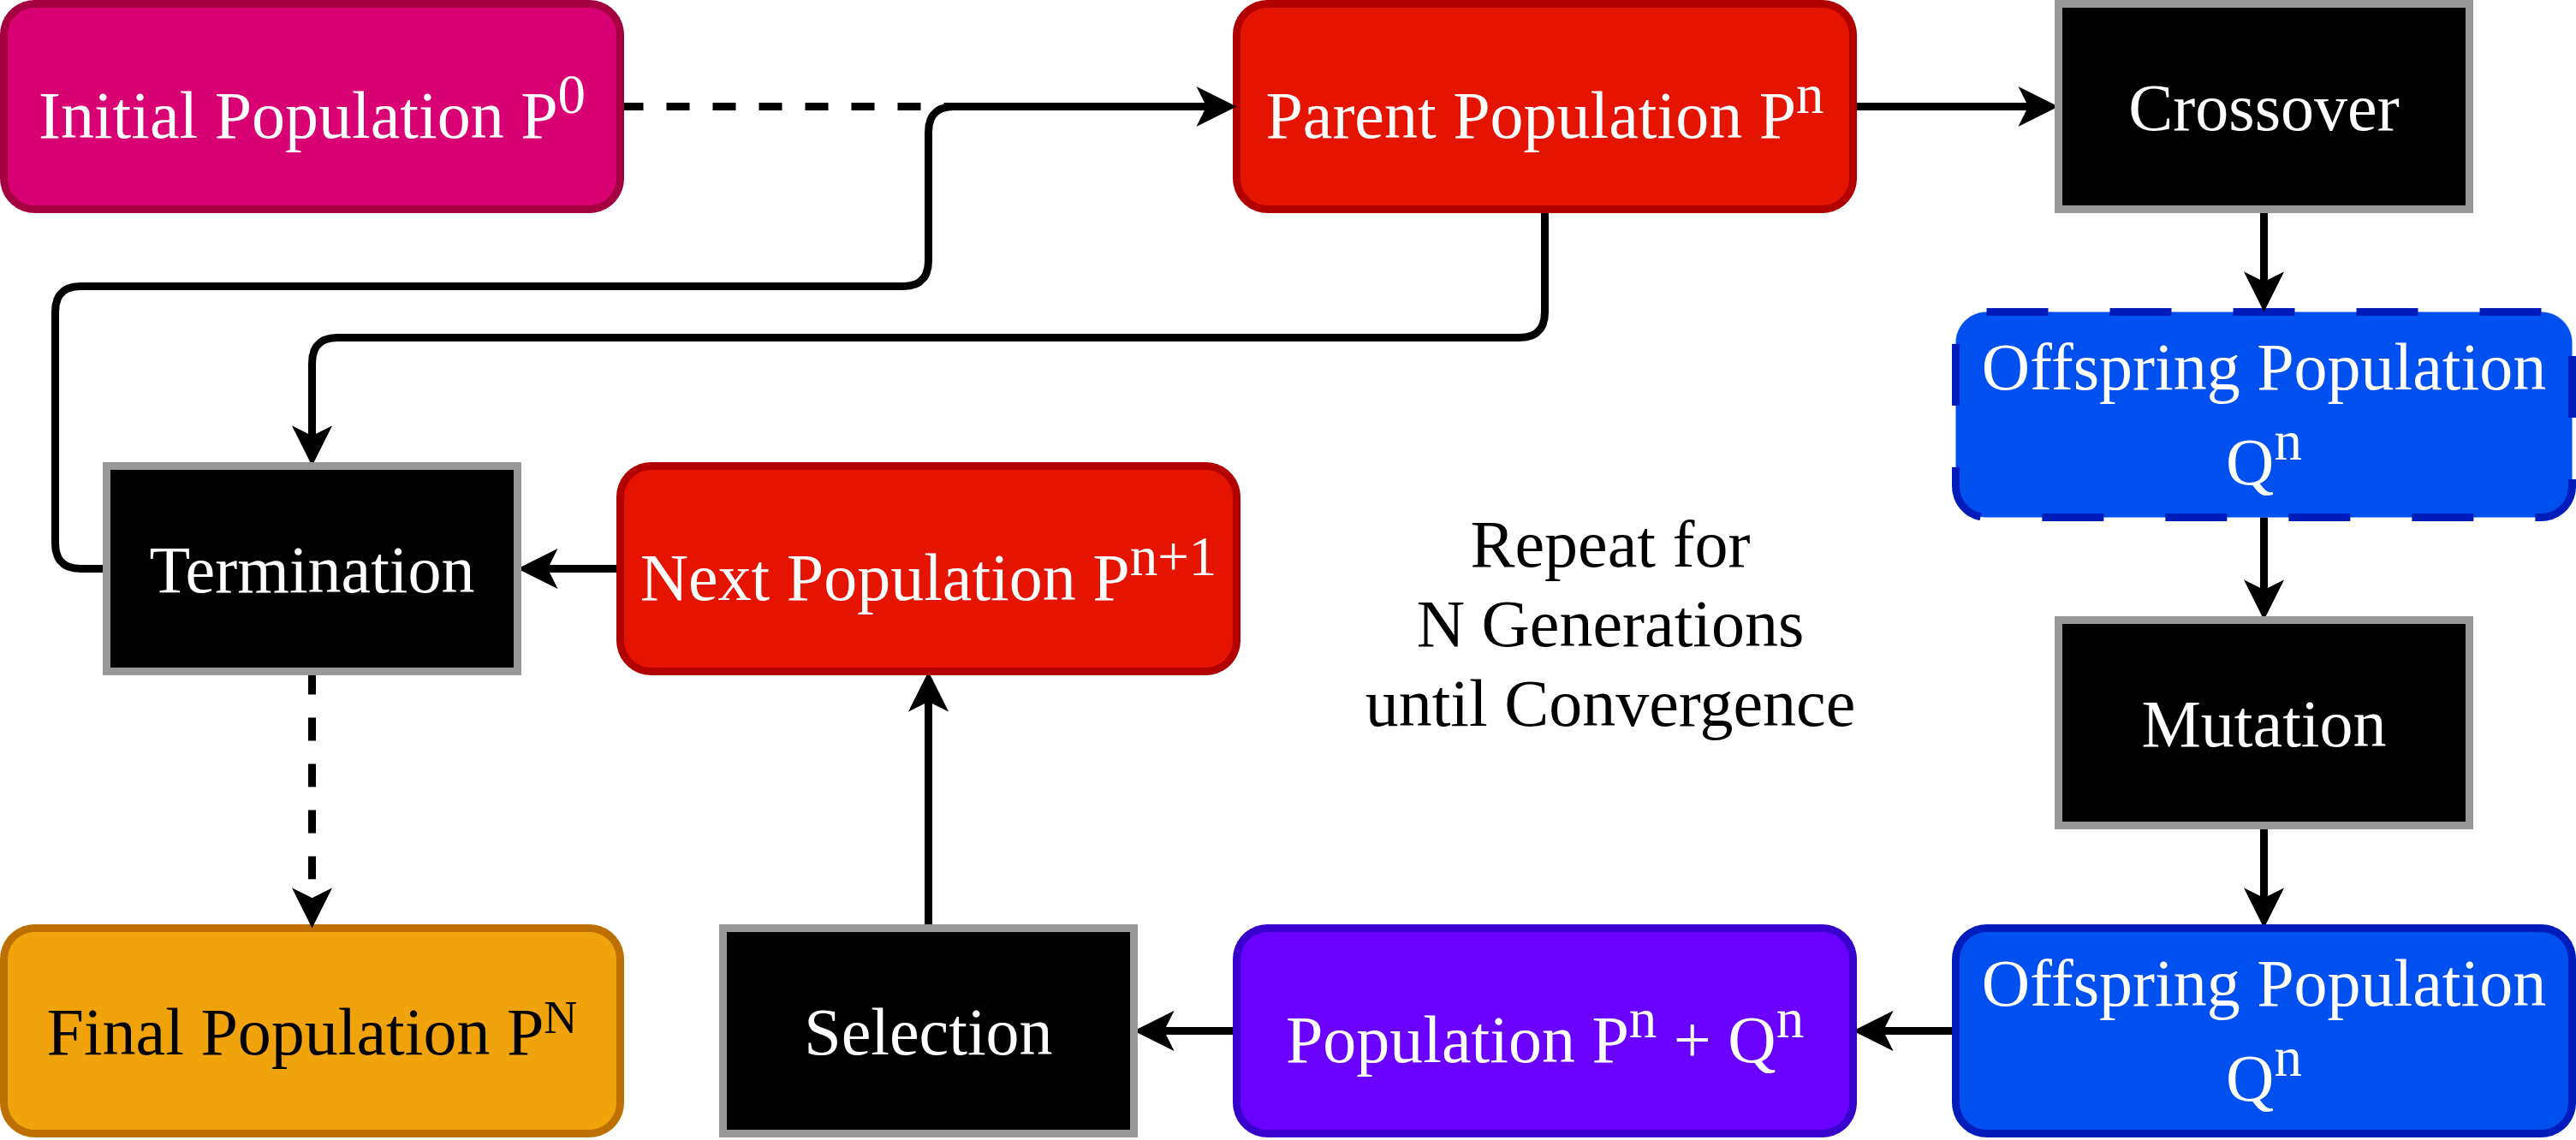
\includegraphics[width = \figurewidth]{figs/genetic_algorithm.png}
	\caption{}
	\label{fig:ga_schematic}
\end{figure}

%\begin{multicols}{2}

The operators used in \gls{ga} are Crossover, Mutation, Selection, and Termination. These operators take a population of solutions as inputs and return a population of solutions as outputs. \gls{ga} operators are defined in detail as follows:

\begin{description}
	\item[Crossover] The crossover operator batches population $P^n$ of size $M$ into pairs. Each pair begets two child solutions with each parent contributing roughly half of the genes of each child. This results in a child population $Q^n$ of size $M$.
	\item[Mutation] The mutation operator iterates through $Q^n$ and randomly resets the value of genes with a given probability.
	\item[Selection] The selection operator serves to determine which solutions of the combined population $P^n \cup Q^n$ will form $P^{n + 1}$.
	\item[Termination] The termination operator determines whether or not to produce another generation. Termination should occur after convergence.
\end{description}

\gls{ga} allows for the solution of an integer or mixed-integer problem without computing every possible combination of integer values. While optimal solvers are guaranteed to find the global optimum (subject to tolerances) \gls{ga} is not. \gls{ga} does not allow for computation of the optimality gap at any time, including at convergence. The likelihood of \gls{ga} arriving at the optimum increases asymptotically with the ratio of $M$ to the number of genes (variables) in $U$.

\subsection{Non-dominated Sorting Genetic Algorithm}

Extending \gls{ga} to \gls{moo} requires very little adjustment of the baseline method. Crossover, mutation, and termination operators remain unchanged. Only the selection operator is altered. Classically, the fitness of solution $U_i$ is determined by the objective function $J = F(U)$. A \gls{moo} problem is defined by a set of objective functions $\hat{F} = \{F_0, F_1, \dots, F_K\}$ which are not weighted relative to one-another and may be contradictory. Evaluating such functions relative to one-another requires introducing the concepts of Non-Domination and Crowding-Distance.

\subsubsection{Non-domination}

Solution $U_i$ dominates solution $U_j$ if and only if $F_k(U_i) \leq F_k(U_j)$ for all $F_k \in  \hat{F}$ and there exists some $\hat{F}' \in  \hat{F}$ where $F'_k(U_i) < F'_k(U_j)$ for all $F'_k \in  \hat{F}'$. In other words, $U_i$ dominates $U_j$ when $U_i$ is at least good in all aspects and better in at least one aspect. In this case, a rational decision maker, when presented with $U_i$ and $U_j$, will always pick $U_i$ regardless of personal priorities. The opposite condition is non-domination which occurs wherever the conditions of domination are not met. Non-domination is common with contradictory objectives such as price and quality. In this case, rational decision makers may disagree based on personal preference, even with identical information. 

A domination front is a set of solutions of the same domination rank. The first front are all solutions which are not dominated by any other solution. Unless all solutions are included in the first front, removing the first front is guaranteed to produce an new non-dominated front which can be called the second front. This process can be repeated until all solutions are assigned to a front as shown in Figure \ref{fig:non_dom_sort}. The rank of a solution is determined by its front and is the primary metric of selection.

\begin{figure}[H]
	\centering
	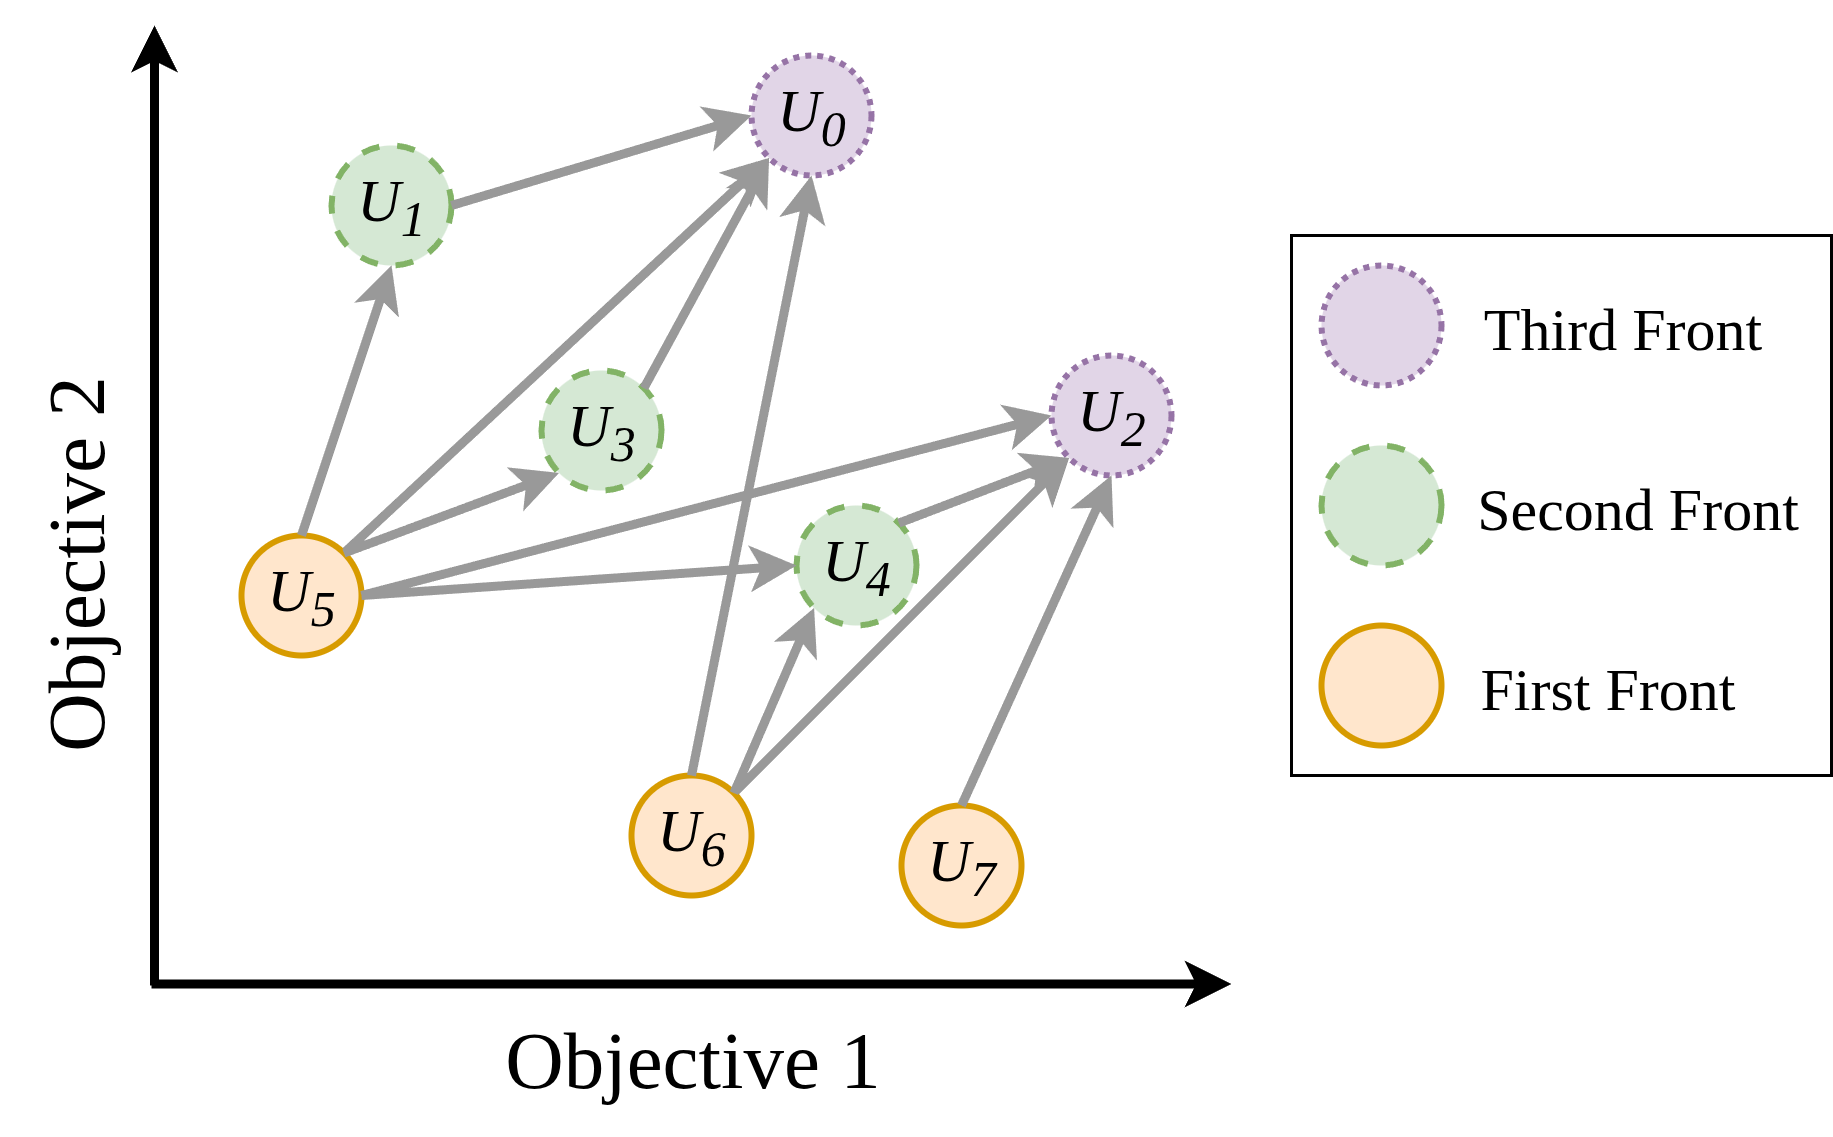
\includegraphics[width = \figurewidth]{figs/non-domination.png}
	\caption{Non-Domination Fronts}
	\label{fig:non_dom_sort}
\end{figure}

\subsubsection{Crowding-Distance}

Many solutions will be of equivalent rank one will often need to pick between solutions of equal rank. When choosing between solutions of equivalent rank, the maintenance of field spread is prioritized. Contribution to field spread is captured in the Crowding-Distance ranking. Crowding-Distance measures the gap in the front which would appear if $U_i$ were removed. Those solutions with the highest resulting gap are prioritized for selection. Each front must have two extrema for each objective. Extrema are awarded a crowding-distance of infinity. Crowding-distance ranking is demonstrated in Figure \ref{fig:crowding_distance}.

\begin{figure}[H]
	\centering
	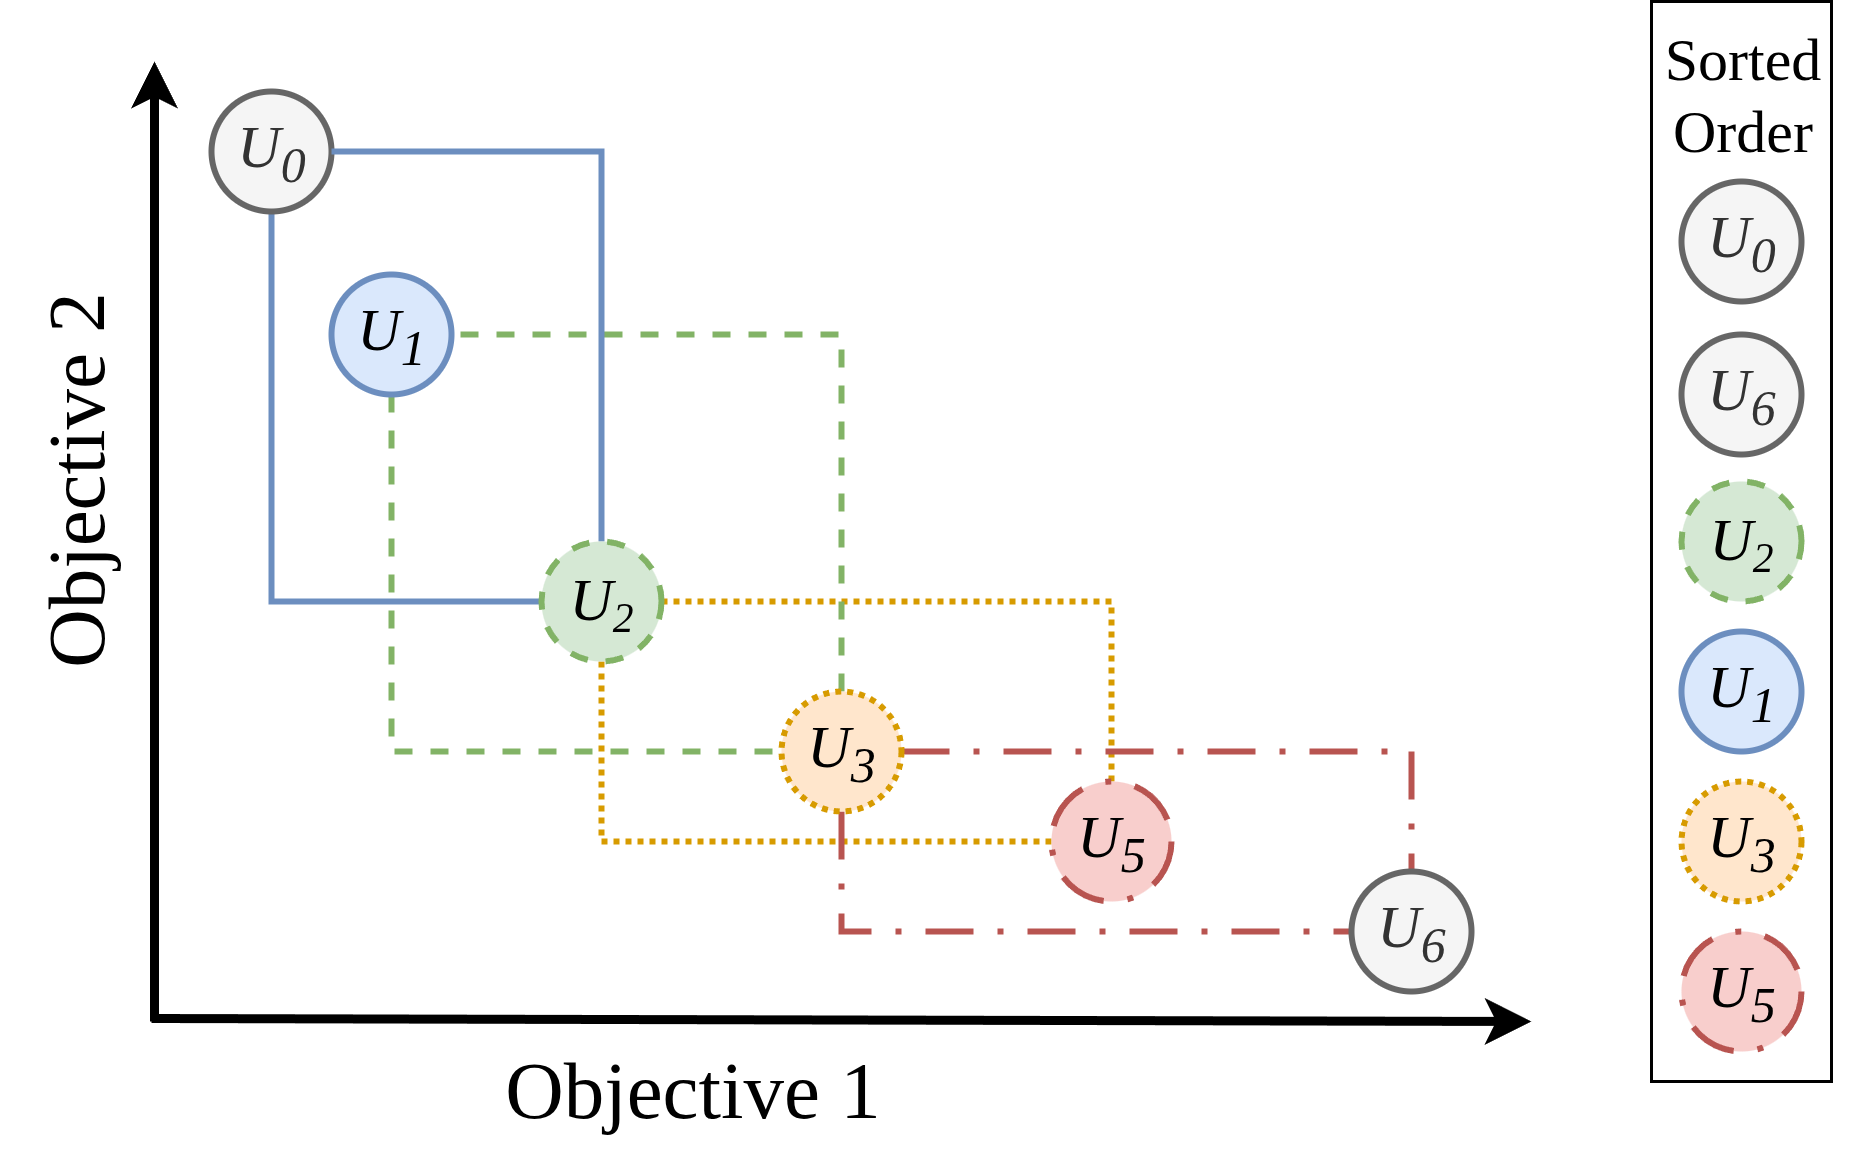
\includegraphics[width = \figurewidth]{figs/crowding-distance_1.png}
	\caption{Example crowding distance ranking. $U_0$ and $U_6$ are given a score of infinity as they are extrema. The remaining points are sorted in descending order based on the size of gap that would be created by their removal.}
	\label{fig:crowding_distance}
\end{figure}

\subsubsection{Selection}

\gls{nsga} calls for Elitist selection. From a combined population of $2 M$ solutions, the best $M$ solutions form the next generation. This is accomplished as follows. First, the solutions of the combined population $P^n \cup Q^n$ are ranked. Iterating through fronts in order, if the size of a front is less than $M - |P^{n + 1}|$ then the entire front is added to $P^{n + 1}$. If the size of the front is greater than $M - |P^{n + 1}|$, then the solutions in front are sorted for crowding-distance and solutions are added in order until $|P^{n + 1}| = M$.

\subsection{Defining the \gls{vsfmp}}

The \gls{vsfmp} concerns the optimization of strategic purchasing decisions for a bus fleet or other vehicle fleet with rigidly scheduled service trips. The problem is solved by finding an assignment of vehicles to service trips and supply events and an assignment of supply equipment to supply events. The assignment must account for the cost and feasibility of transitioning from one service trip or supply event to another. Purchasing and installing equipment incurs up-front costs which scale with the amount purchased while operating costs scales with time worked and energy expended. The method presented is generic and specific cost functions will be provided for case studies.

\subsection{Encoding the \gls{vsfmp}}\label{sec:ebrp}

Posing the \gls{vsfmp} for \gls{ga} requires encoding the problem onto chromosomes. This is non-trivial due to the nature of the problem. Previous schema are presented in \cite{Rogge_2018_AE, Li_2020_JAT, Yao_2020_SCS}. Where \cite{Li_2020_JAT} is a straightforward implementation, the others reformulate the \gls{vsfmp} to better fit \gls{ga}. The approach of \cite{Rogge_2018_AE} is to group service trips into blocks (tours) and solve a simplified \gls{milp} while the approach of \cite{Yao_2020_SCS} is to encode trip order into chromosomes and use a heuristic assignment method. The proposed method draws inspiration from both. First a graphical structure is devised which serves as the chromosomes indirectly encoding vehicle tours and allowing for straightforward crossover and mutation. Following this, an assignment heuristic is utilized for the reduced problem. This approach provides a more direct link between genetic material and fitness compared to \cite{Yao_2020_SCS} and a more direct crossover and mutation compared to \cite{Rogge_2018_AE}. The method is also generic and inherently suited for \gls{moo}.

The encoding scheme is built around three structures. The first structure is the Successors Graph which stores the successor activity for each trip (another trip or return to depot). The second is the Vehicle Type Map which assigns a vehicle type to each trip. The third is the Port Type Map which assigns a supply port type to each trip. These structures constitute the genetic material. The structures must be co-optimized as there is substantial interaction between them.

\subsubsection{Successors}

A bus network schedule is a set of trips $V$ where each trip is defined by start and finish times and locations and energy requirements. Given knowledge of the time required to transition between route terminals and depots, it is possible to construct Trips Graph $G = \{V \cup D, E\}$ where $D$ contains all depots and $E$ contains all possible transit legs.

Tours may be stored by storing the successor activity to each trip. For a valid tours assignment, all trips $v_i \in V$ must have exactly one successor. This successor may be another trip or a depot. Depots $d_i \in D$ may have many successors but it is not necessary to store these. The predecessor-successor links form the edges of a directed Successors Graph $G^S = \{V \cup D, S\}$ where $S \in E$ are the edges which form the tours. Edges in $S$ may only originate with a trip in $V$ but may terminate with a trip in $V$ or a depot in $D$. There are many possible permutations of $S$ for any realistically scaled $G$. The set of possible permutations of $S$ is $\hat{S}$ and much of the work of solving the \gls{vsfmp} is finding the subset of $\hat{S}$ that corresponds the Pareto Front in an efficient manner. $S^T = \{i\ \forall\ (i, j) \in S\}$ is the set of tail nodes for the edges in $S$ and $S^H = \{j\ \forall\ (i, j) \in S\}$ is the set of head nodes for the edges in $S$. $S^T$ must contain all trips in $V$ but $S^H$ need not contain all trips in $V$.

For each $S_i \in \hat{S}$ there is a corresponding Predecessors Set $\Pi_i$ whose edges are $\{(j, i)\ \forall\ (i, j) \in S\}$ such that the graph formed from the combination of $S^i$ and $\Pi^i$ is undirected. $\Pi^i$ is used to recover tours. Starting from depots, \gls{bfs} is used to recover all tours up to the point that predecessors are exhausted. Since tours must start and finish at the same depot, each tour starts at the same depot at which it finishes.

Consider the simple Trips Graph shown in Figure \ref{fig:trips_graph}. The simple Trips Graph defines a network which operates two routes for three trips each.

\begin{figure}[H]
	\centering
	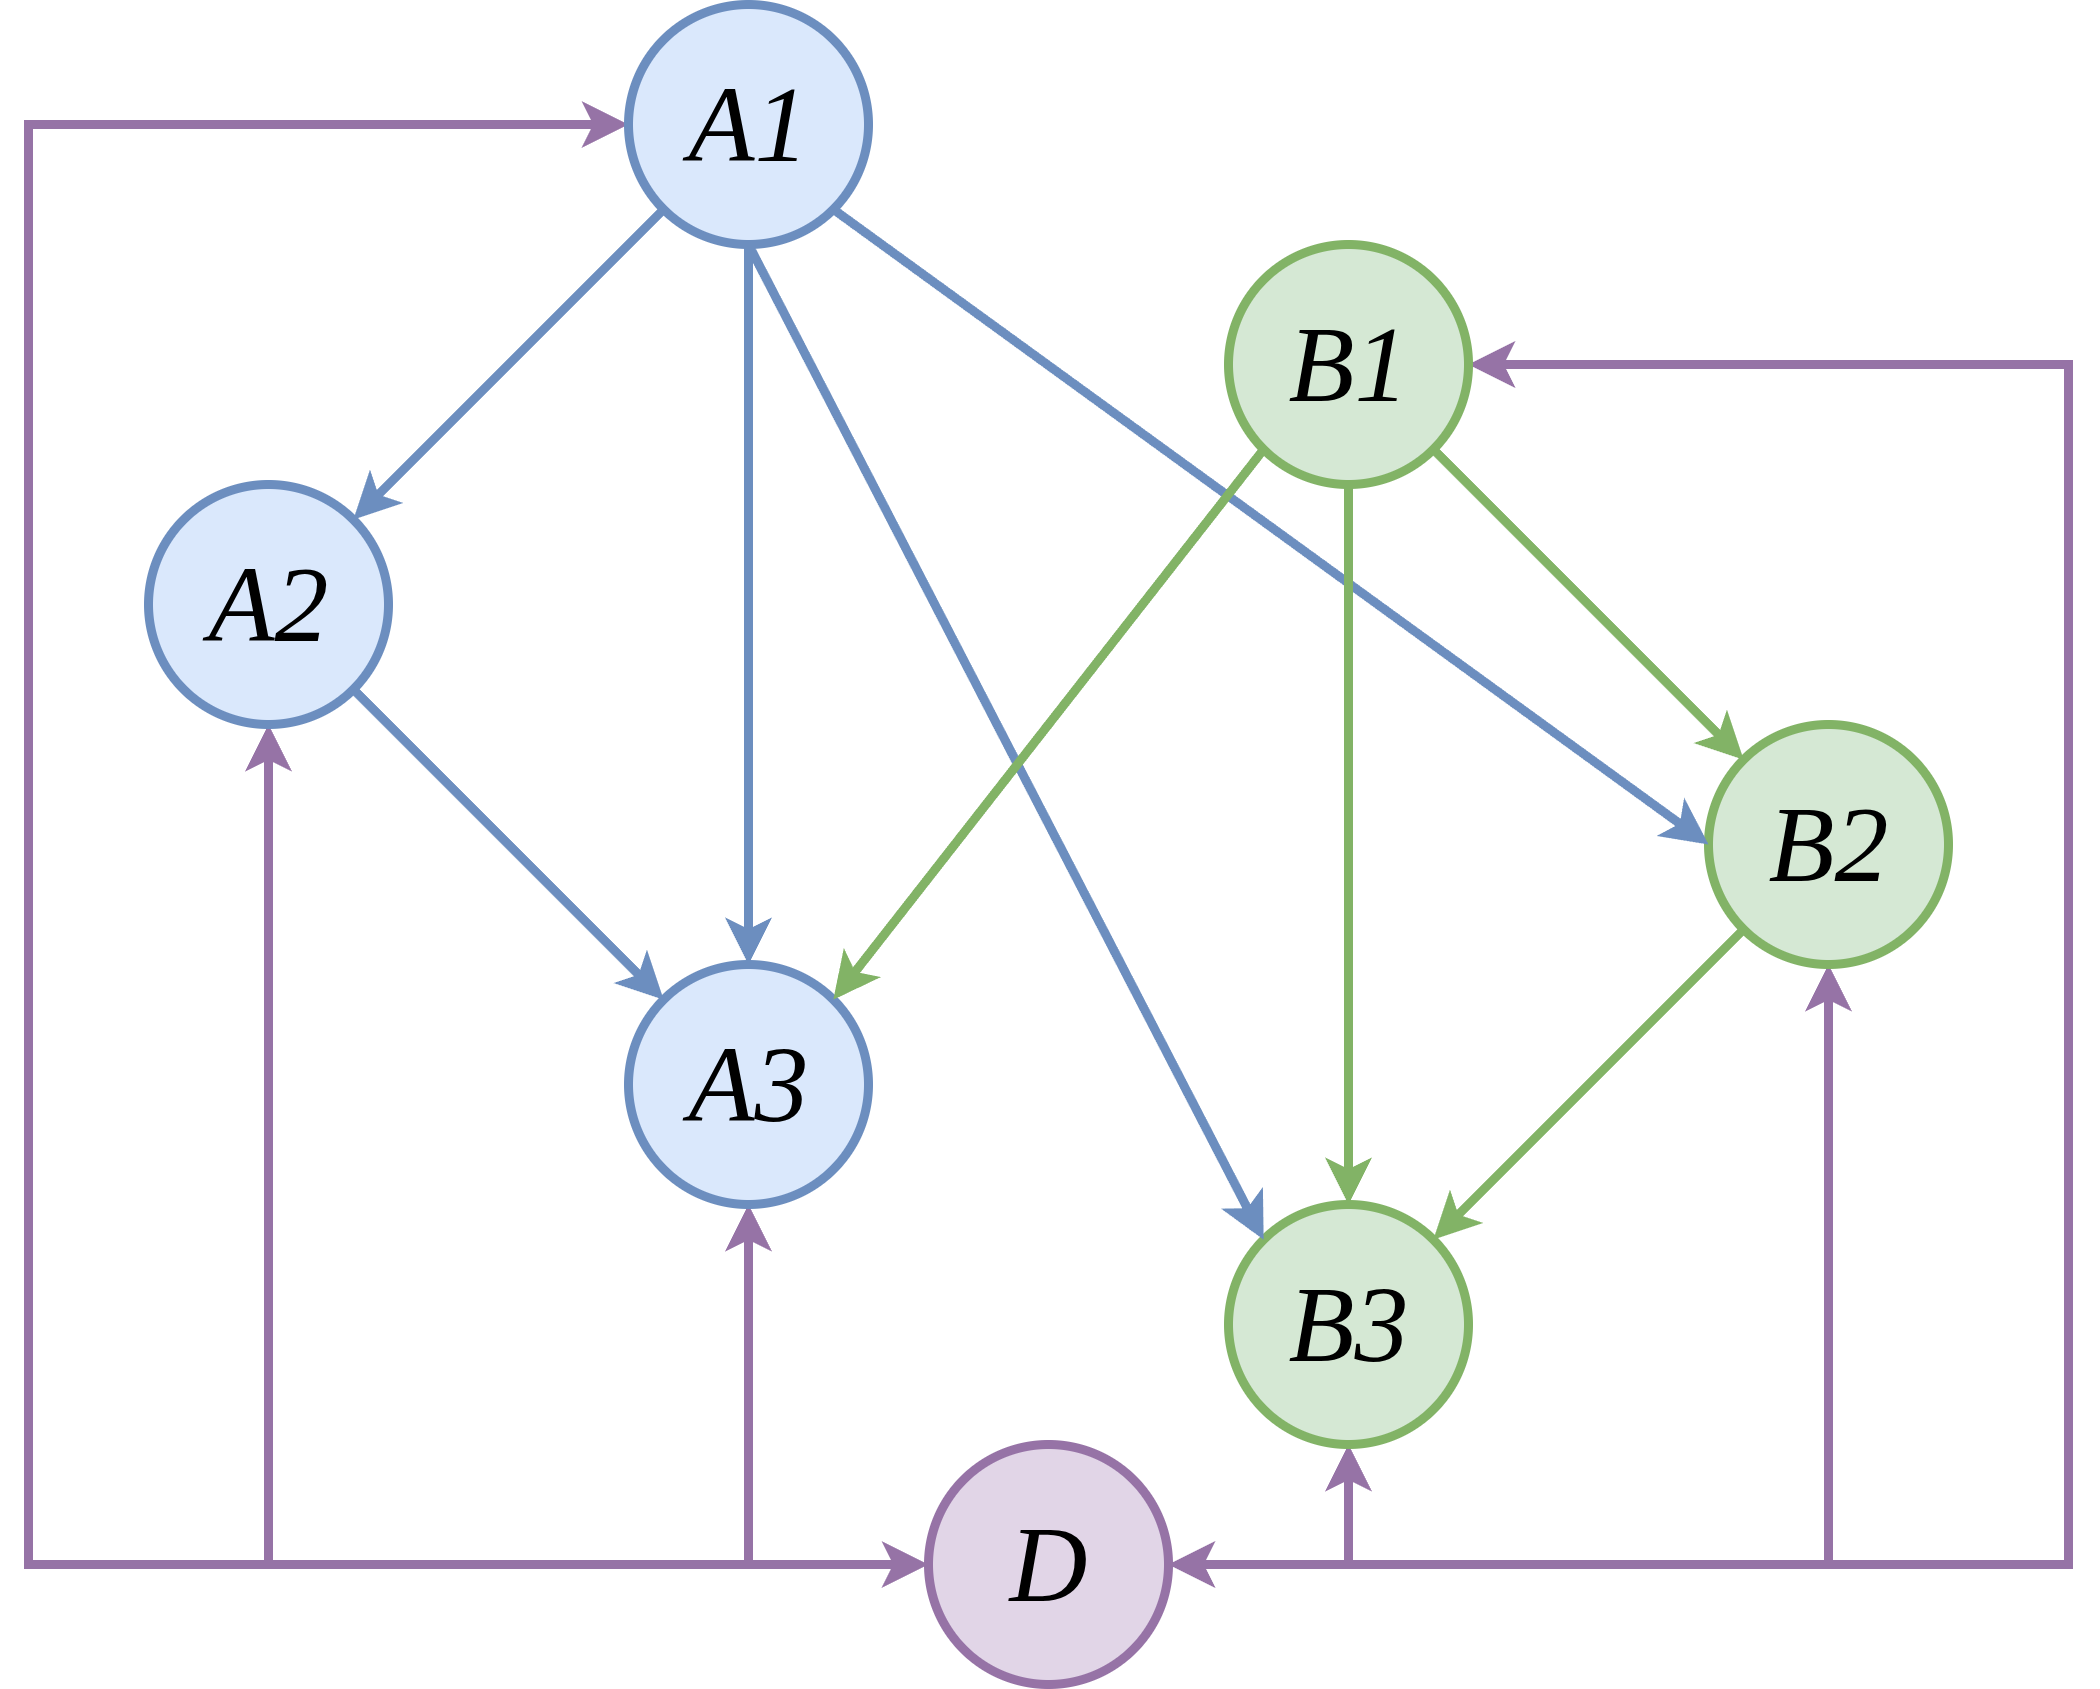
\includegraphics[width = .5\linewidth]{figs/trips_graph.png}
	\caption{}
	\label{fig:trips_graph}
\end{figure}

A valid Successors and the resulting Predecessors are provided in Figure \ref{fig:successors_predecessors}.

\begin{figure}[H]
	\centering
	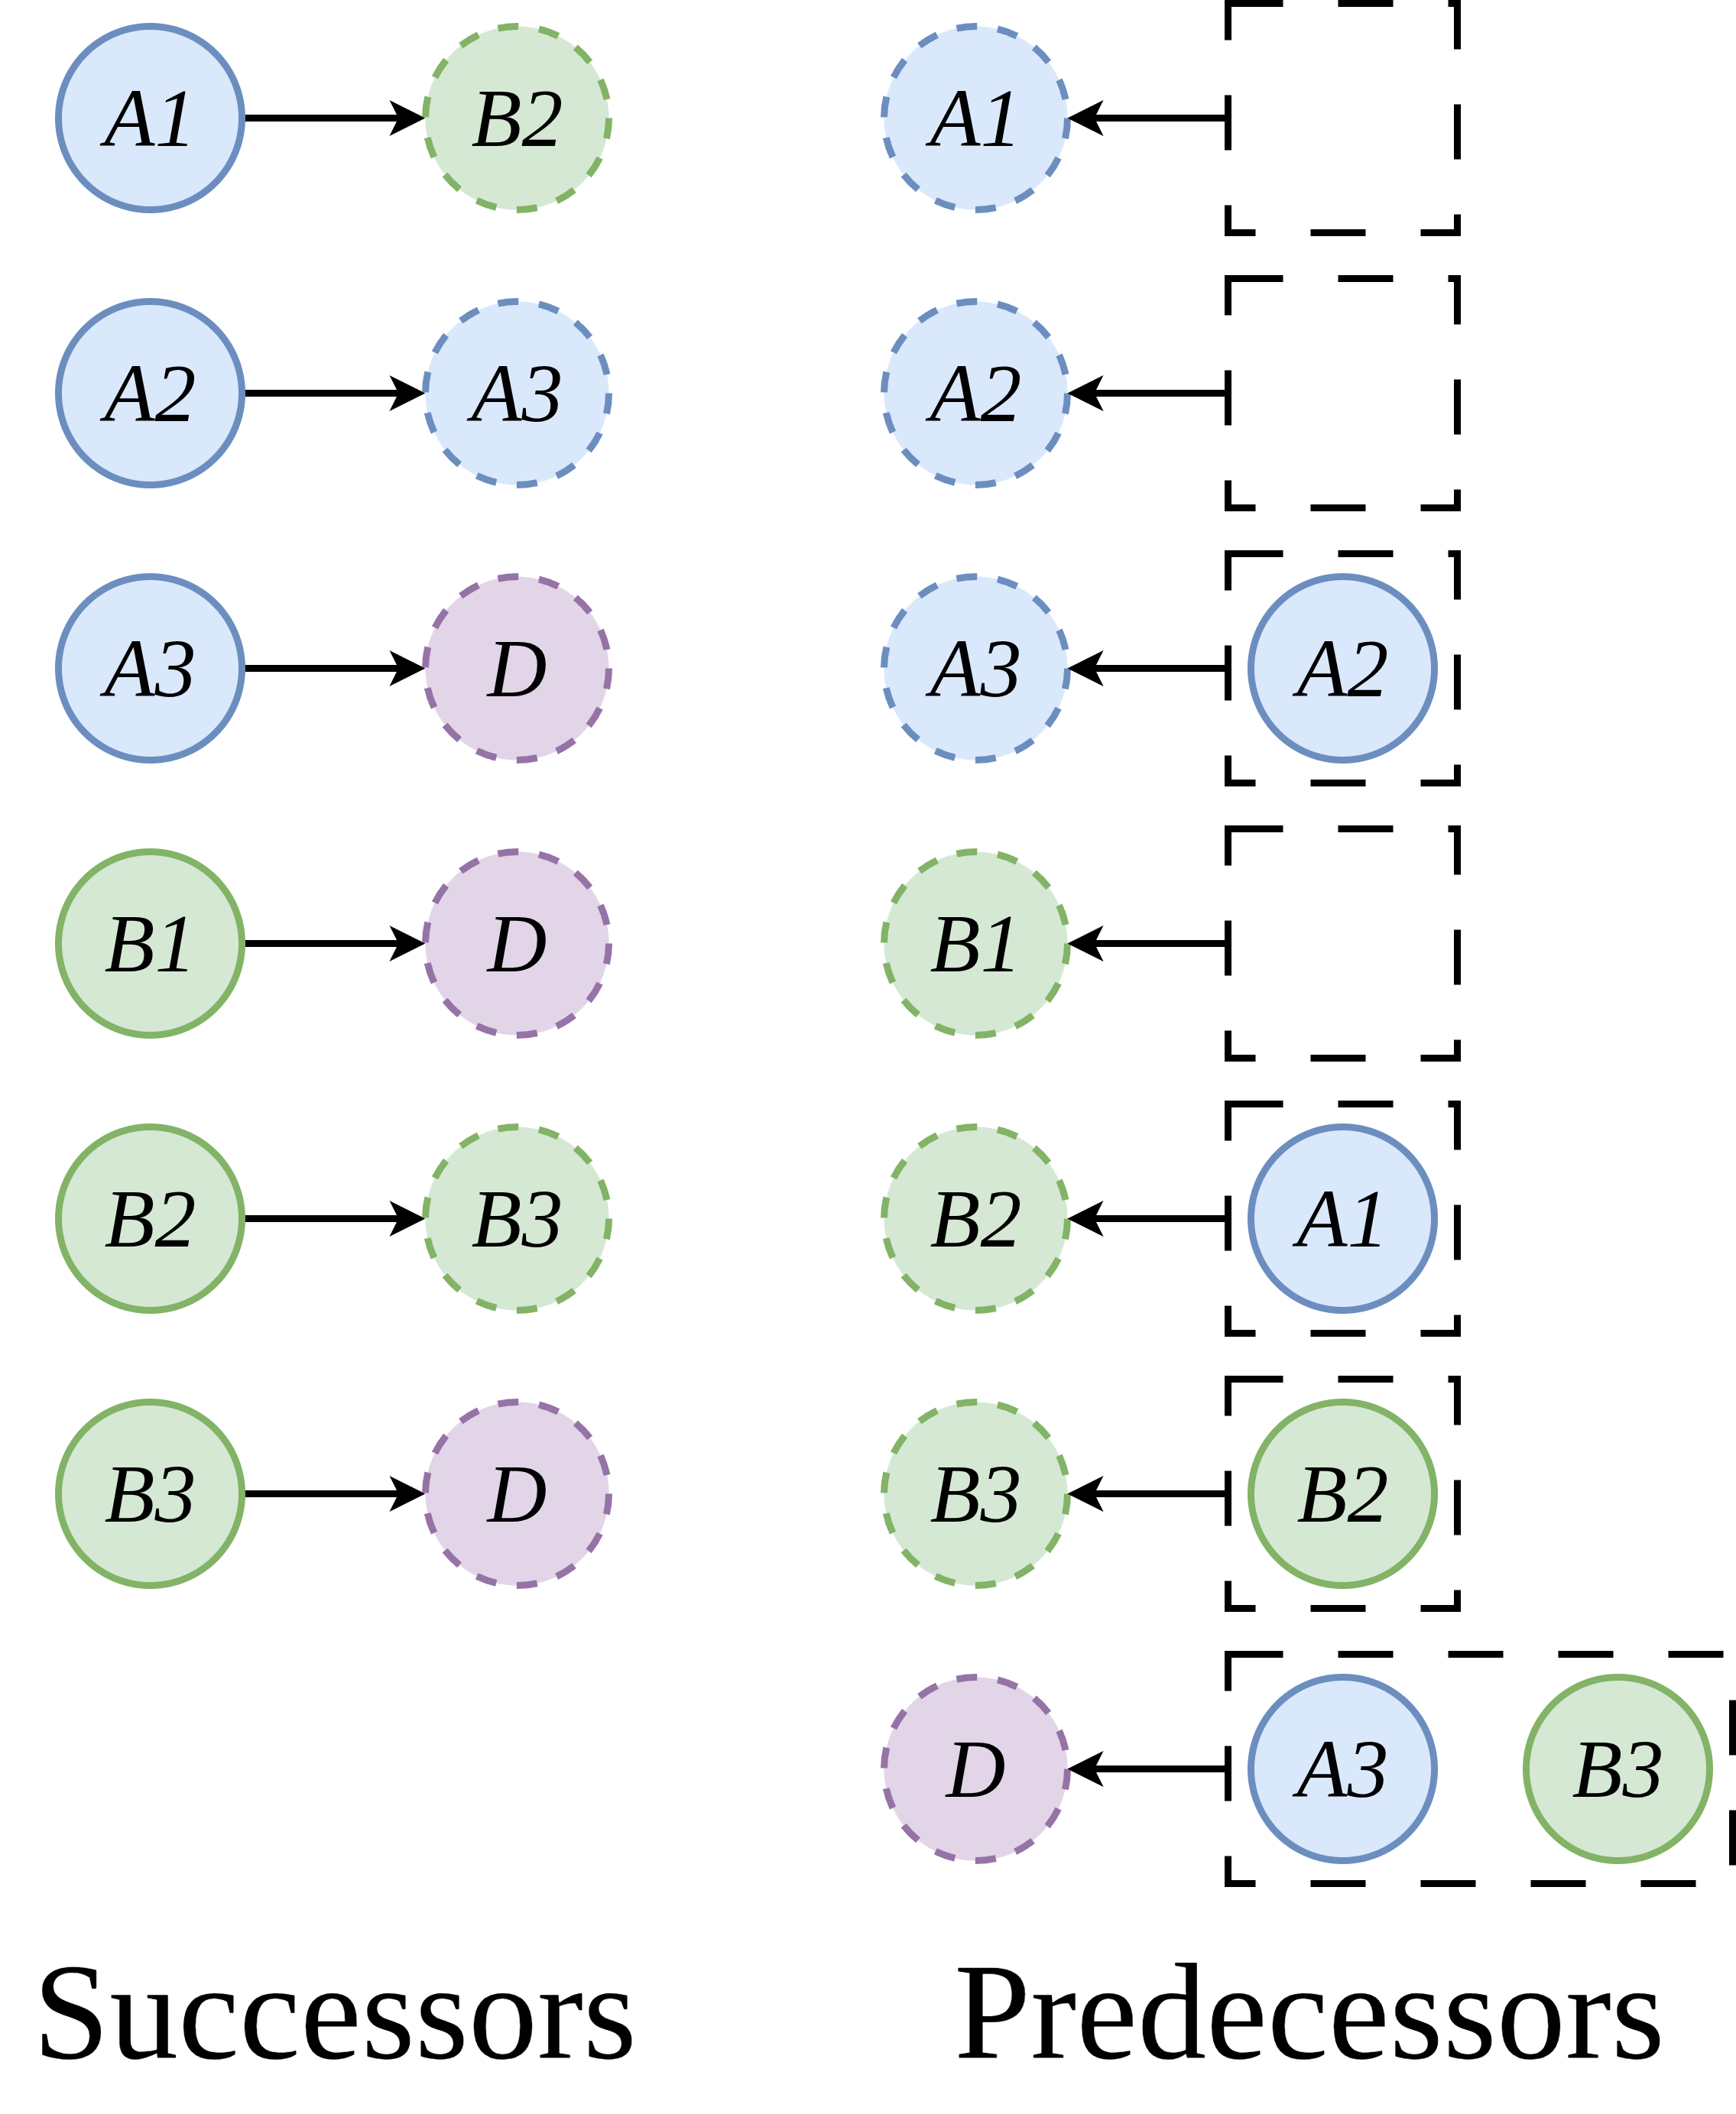
\includegraphics[width = .5\linewidth]{figs/successors_predecessors.png}
	\caption{}
	\label{fig:successors_predecessors}
\end{figure}

Which leads to the set of tours shown in Figure \ref{fig:tours}.

\begin{figure}[H]
	\centering
	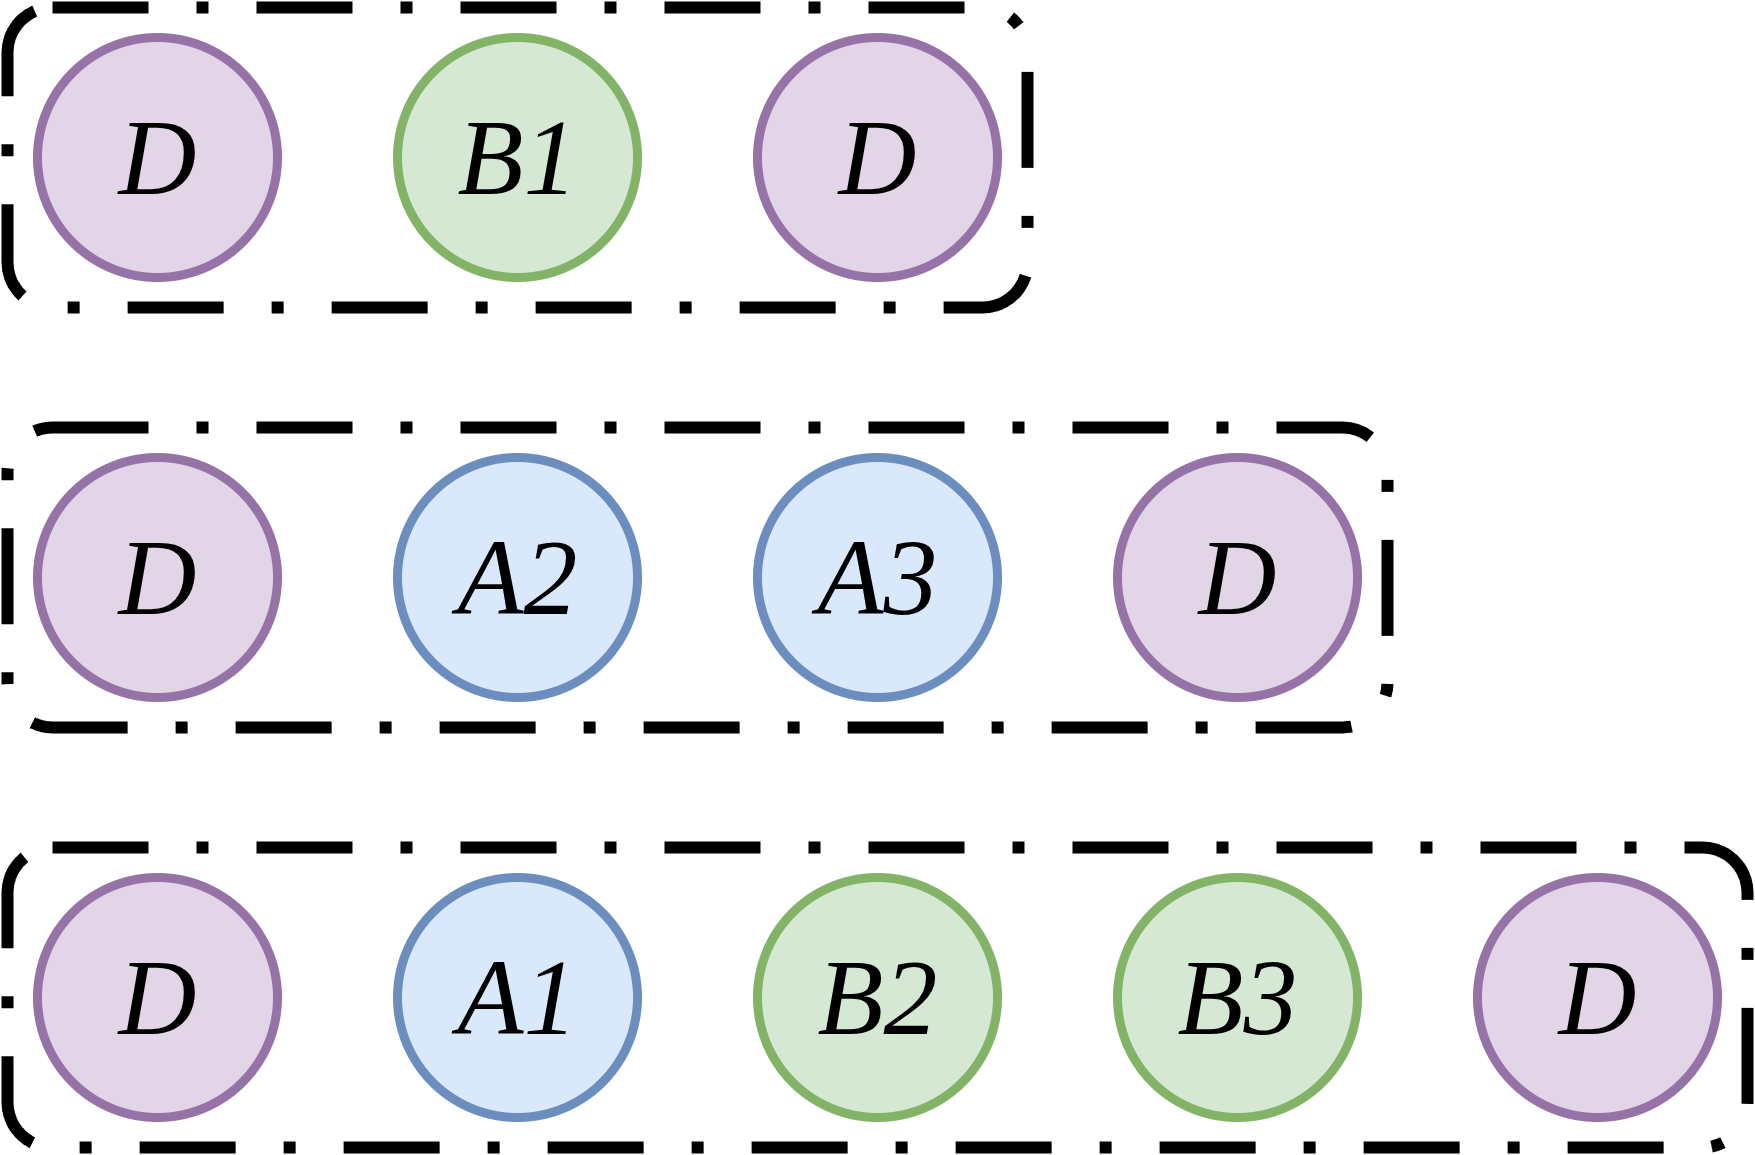
\includegraphics[width = .5\linewidth]{figs/tours.png}
	\caption{}
	\label{fig:tours}
\end{figure}

The Successors structure leads directly to the tours. Although this encoding is more memory intensive than a simple ordering it allows for simple and robust Crossover and Mutation operators.

\subsubsection{Vehicle Types}

The Vehicle Type Map is a simple map linking trips in $V$ to vehicle types in the set $B^V$ $A^V: V \rightarrow B^V$. Each trip in $V$ receives an assigned vehicle type in initial population generation. After tours are reconstructed, many tours will contain trips with multiple bus-type assignments. In this case, there is a "vote". If one bus type attains a plurality within the tour, the tour is assigned that bus type. Ties are broken by order of appearance. Following the vote, all trips in the tour are assigned the selected vehicle type. This process is shown in Figure \ref{fig:voting}.

\begin{figure}[H]
	\centering
	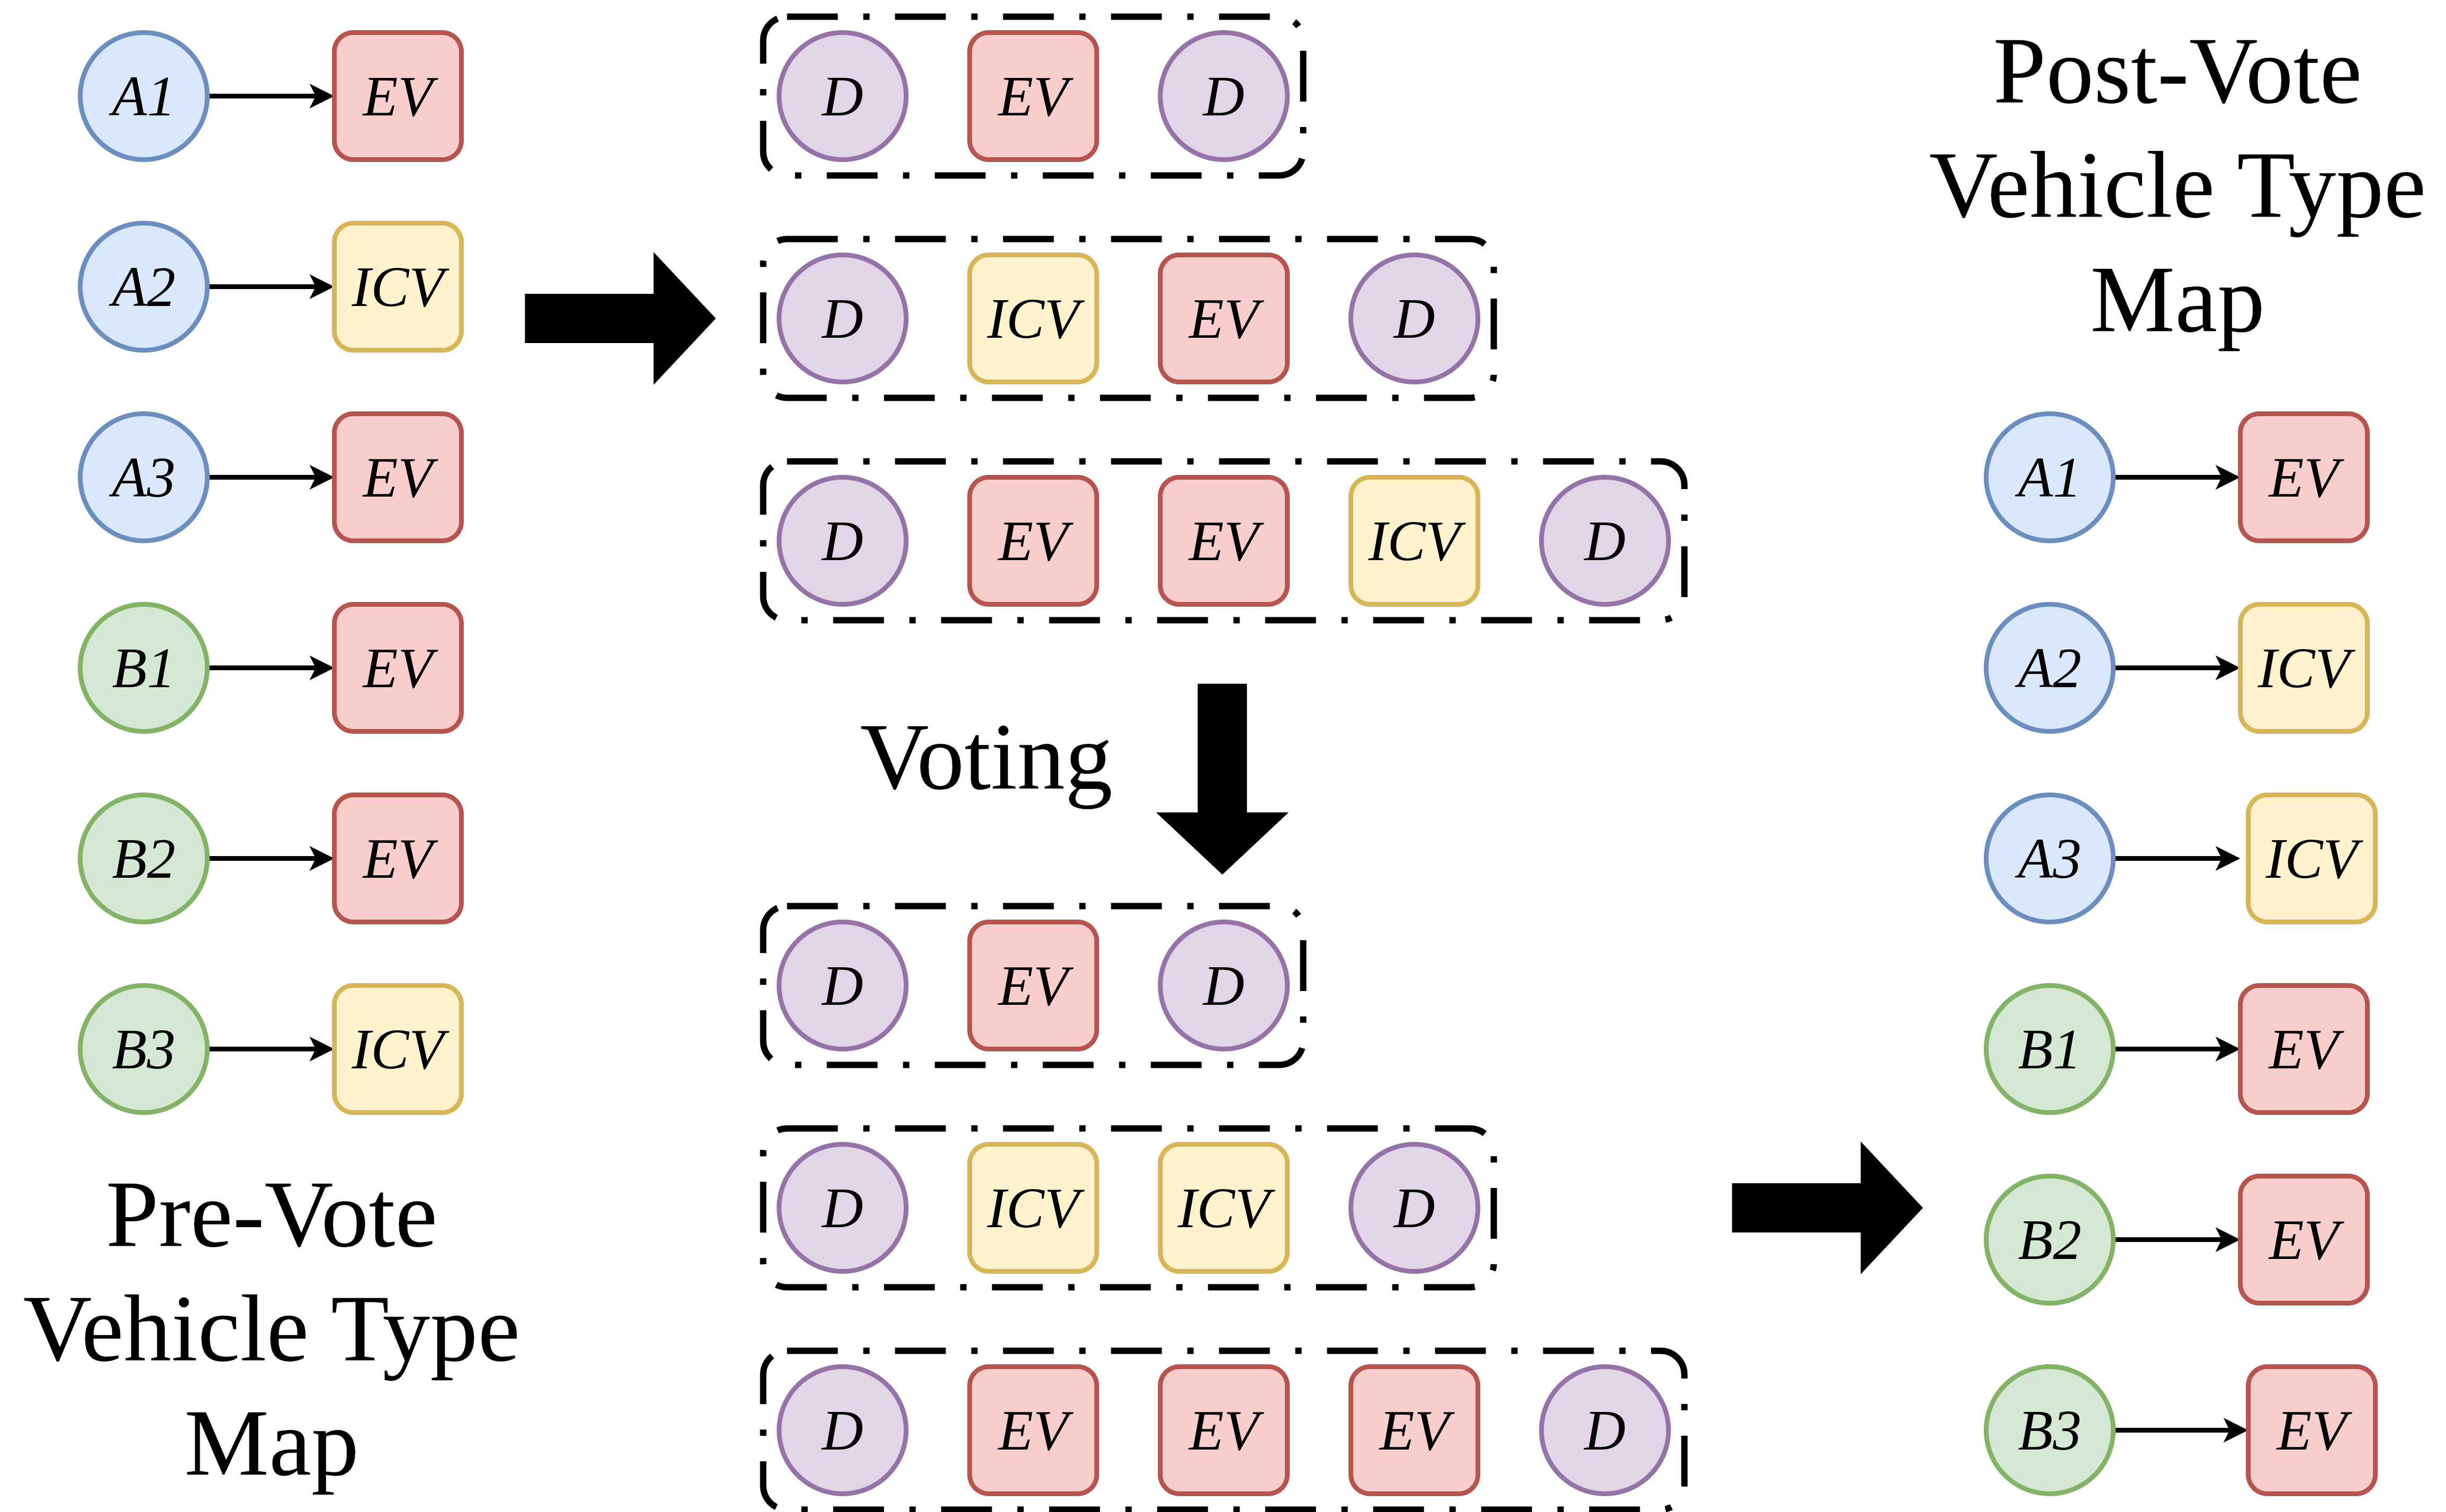
\includegraphics[width = \linewidth]{figs/voting.png}
	\caption{}
	\label{fig:voting}
\end{figure}

\subsubsection{Port Types}

The Port Type map $B^P$ $A^P: V \rightarrow B^P$ functions similarly to the Vehicle Type map. When the Port Type map is initialized, each assignment is a valid assignment for the type of vehicle assigned to the same trip. When the vehicle type for a tour is determined, the port type for the tour is the predominant port type among the vehicles of the selected vehicle type included in the tour. Thus the port type selected for a tour will always be compatible with the vehicle type.

\subsection{Assignment Heuristic}

Having formed the tours and determined vehicle and port types, the problem becomes an assignment problem. This assignment determines which specific bus within a given type will serve a specific tour and which specific port will serve the succeeding supply event.

First, following vehicle type assignment, it is possible that some tours will be infeasible for the vehicle type chosen. In this case, the tours in question are subdivided into two tours with this process repeating until all tours are feasible. Individual vehicles are assigned to tours based on the assigned vehicle type using the heuristic defined in Figure \ref{fig:bus_assignment}.

%\end{multicols}
\begin{figure}[H]
	\centering
	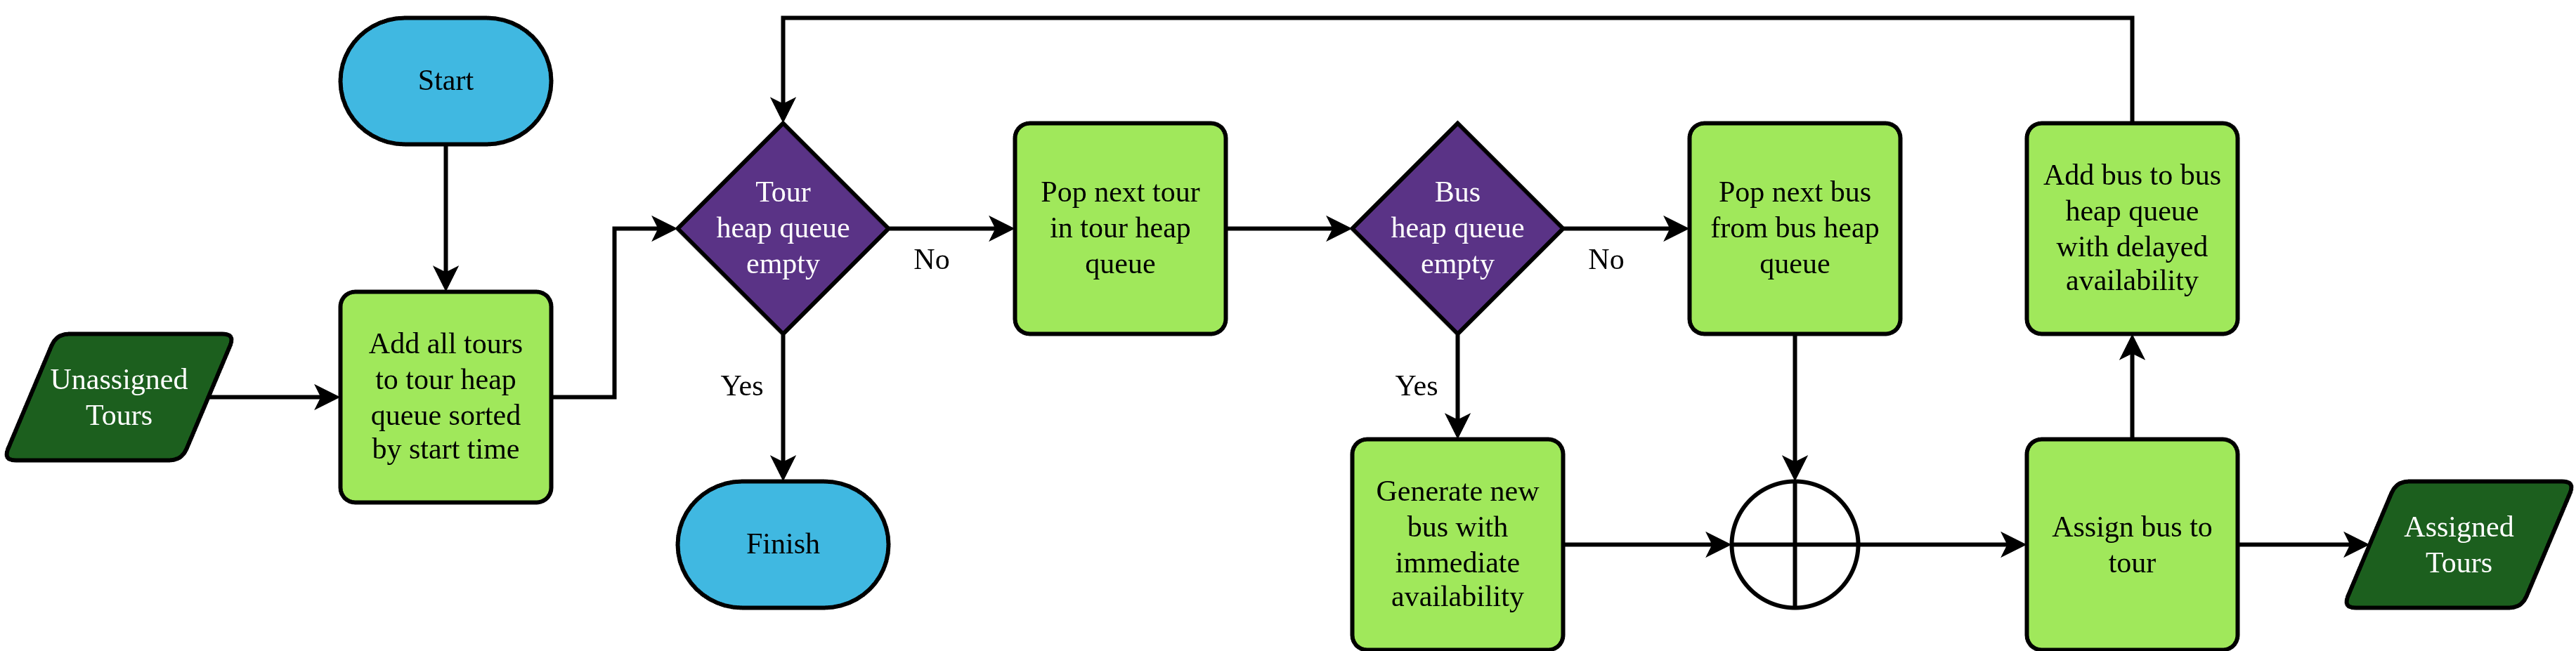
\includegraphics[width = \linewidth]{figs/bus_assignment_1.png}
	\caption{}
	\label{fig:bus_assignment}
\end{figure}
%\begin{multicols}{2}

The process shown in Figure \ref{fig:bus_assignment} pertains to a fleet of a single vehicle type but can be easily extended to multiple vehicle types by implementing a separate queue fo each vehicle type and choosing from the appropriate queue. The heuristic will result in an individual vehicle assigned to each tour and a required number of vehicles for each type.

Having assigned individual vehicles to tours, supply equipment can be assigned to the supply events which follow the tours. Each tour which terminates at a depot with a supply station will be followed by a supply event (charging or fueling) which must be completed before the vehicle can perform another tour. Supply ports are added and assigned to supply events in a similar manner to the vehicle assignment. The main differences are that where tours are sorted by start time, supply events are sorted by finish time.

\subsection{Custom Genetic Operators}

The unique encoding scheme introduced in Section \ref{sec:ebrp} requires custom genetic operators to function. The specific forms of initial population generation and the Crossover and Mutation operators required are discussed in the following sections.

\subsubsection{Initial Population}

The initial population is generated by generating $M$ random configurations of $S$ and $A$. Generating a valid random configuration of $S$ requires that each trip in $V$ have exactly one predecessor and successor in $V \cup D$. This is accomplished by iterating through the trips in $V$ in random order and, for each trip, randomly choosing a successor from the set of possible successor trips and depots. Each time a successor is assigned the successor trip is no longer able to be selected for any other trip. $A$ is generated by random selection of vehicle types in $B$ for each trip in $V$. The Vehicle Type and Port Type maps are also randomly generated. For each trip in $V$, a vehicle type is selected from a weighted distribution among the types in $B^V$ and a valid port for said vehicle type is randomly selected from $B^P$. 

\subsubsection{Crossover and Mutation}

Crossover is accomplished by the exchange of genetic material among randomly selected pairs of parents from $P^n$ with each parent paired exactly once. For parents $a$ and $b$ children $c$ and $d$ are formed by the crossover process. Child $c$ is formed by copying parent $a$ and subsequently incorporating selected genetic material from parent $b$. Child $d$ is formed by copying parent $b$ and subsequently incorporating selected genetic material from parent $a$. The contribution to child $c$ from parent $a$ is referred to as the original material and the contribution from parent $b$ is referred to as the crossover material and \textit{vice versa} for child $d$. In order to minimize duplicated work the Crossover and Mutation operators are merged. If the mutation probability is greater than zero, randomly selected genes are changed within the crossover material before crossover happens. Crossover and Mutation are accomplished differently for Successors and Vehicle/Port Types.

\paragraph{Successors} Crossover of successors is accomplished by the random swapping of edges in the Successors Graph among pairs of parents from $P^n$. As the Successors Set contains an edge for each trip in $V$, each $S \in \hat{S}$ will have the same number of edges with the same tail nodes. Edges are selected for crossover randomly with a probability of $\phi^c$ which is $0.5$ by default. Mutation occurs with probability of $\phi^m$ and involves swapping the selected edge with another edge in $E$ with the same tail node. On its own, this will often create a situation where one node serves as successor to multiple other nodes, thus appearing in multiple tours. This is invalid and requires adjustment of $S$. Consider the insertion of $(t, h)$ from $S_b$ into $S_a$. $S_a$ will contain an edge $(t, h')$ which contains the same tail node and, a possibly different head node. $S_a$ may also contain an edge $(t', h)$ which has the same head node as the inserted edge but a different tail node. This can create a conflict. The following operations are used depending on what potential conflicts exist.

\begin{description}
	\item[Clean Insert] If $(t', h) \notin S_a$ ($h$ is not the successor for any trip) then $(t, h)$ can replace $(t, h')$ without causing a conflict. In this case $h'$ no longer serves a a successor to any trip.
	\item[Replacement] If $(t', h) \in S_a$ ($h$ is the successor for another trip $t'$) and $(t', h')$ is not a possible edge then $(t, h')$ is dropped from $S_a$ and $S_a$ gets $(t, h)$. In this case $h'$ no longer serves a a successor to any trip and $t'$ no longer has a successor trip.
	\item[Swap] If $(t', h) \in S_a$ ($h$ is the successor for another trip $t'$) and $(t', h')$ is a possible edge then a swap occurs and $S_a$ gets $(t, h)$ and $(t', h')$.
\end{description}

\paragraph{Vehicle and Port Types} Each solution in $U_i \in P^n$ contains a unique vehicle type mapping $A^V$ and port type mapping $A^P$. Crossover is straightforward. A set of trips are designated for crossover and the vehicle types and port types are swapped between the parents. Vehicle and port types are swapped simultaneously and for the same selected trips in order to maintain valid port assignments.

\subsection{Constraint Handling}

It is possible for a valid solution to be in violation of some specified constraint. An example may be a limit on expenditures or fleet size. In this case, a compliant-first approach is used. Non-compliant solutions are given ranks which are higher than all compliant solutions. Thus, non-compliant solutions are able to be selected only if there are fewer than $M$ compliant solutions from $P^n + Q^n$.

\subsection{Termination}

A downside of \gls{ga} is that it is not possible to know whether or not a global optimum has been attained. Traditionally, convergence criteria are used for termination. For single-objective optimization, convergence can be determined by the evolution of the best or average value in the population. For Pareto optimization, this method can be misleading. Meaningful expansion of the Pareto front can manifest as no change ot the average or even a reversion. As such, the termination criteria used herein are a minimum number of generations $N^-$, a maximum number of generations $N^+$, and a child survival threshold. As the Pareto front advances, it becomes increasingly unlikely that child solutions will dominate their parents and, as such, be included in the subsequent generation. Thus, between the minimum and maximum number of generations, iteration terminates when fewer than a given number of child solutions survive to the next generation for a given number of consecutive generations.

\subsection{Run-Time Complexity}

The time-complexity of \gls{ga} and \gls{nsga} is known to scale as $O(MN)$ where $N$ is the number of generations and $M$ is the population size. Run-time is, thus, bounded by $O(MN^-)$ and $O(MN^+)$ which may be a large range. Because $N$ is not pre-determined and termination follows convergence the practical run-time is difficult to estimate.

Run-time is most meaningfully impacted by the scale of the Trips Graph $G$ including number of trips in $V$ and the number of feasible connections in $E$. This impact is felt in fitness evaluation, Crossover, and Mutation, and impacts the number of generations required for convergence $N$. Fitness evaluation requires finding tours which relies on \gls{bfs} thus scaling with $|V| + |E|$. All other operations including vehicle and port assignment scale with the number of tours and can be estimated as scaling with $|V|$. Crossover and Mutation require iterating through $S$ so they scale with $|V|$. Ultimately, the expected number of generations before convergence scales with the number of possible configurations of $S$ as well as the inverse of $M$. As will be demonstrated in the Results section, termination often occurs when the product of $M$ and $N$ is on the same order as $|E|$.

Run-time is minimally impacted by the number of objectives. The run-time complexity of the non-dominated sorting and crowding distance sorting algorithms scale with the number of objectives but these operations contribute minimally to overall run-time. Run-time is not impacted at all by the number of vehicle types, number of supply-types, or number of depots.
	\section{Case Studies}\label{sec:case_study}

\subsection{Unitrans}

UC Davis operates a bus network connecting the UC Davis campus to locations around the City of Davis called Unitrans. During academic sessions, this service operates 18 regular routes. The routes are each referred to by a letter. All buses are serviced from a single depot located on nearby the two terminal stations. On a given week the Monday service contains 2,263 individual trips (after merging out and in legs). Start times for the trips are shown in Figure \ref{fig:unitrans_trips}.

\begin{figure}[H]
	\centering
	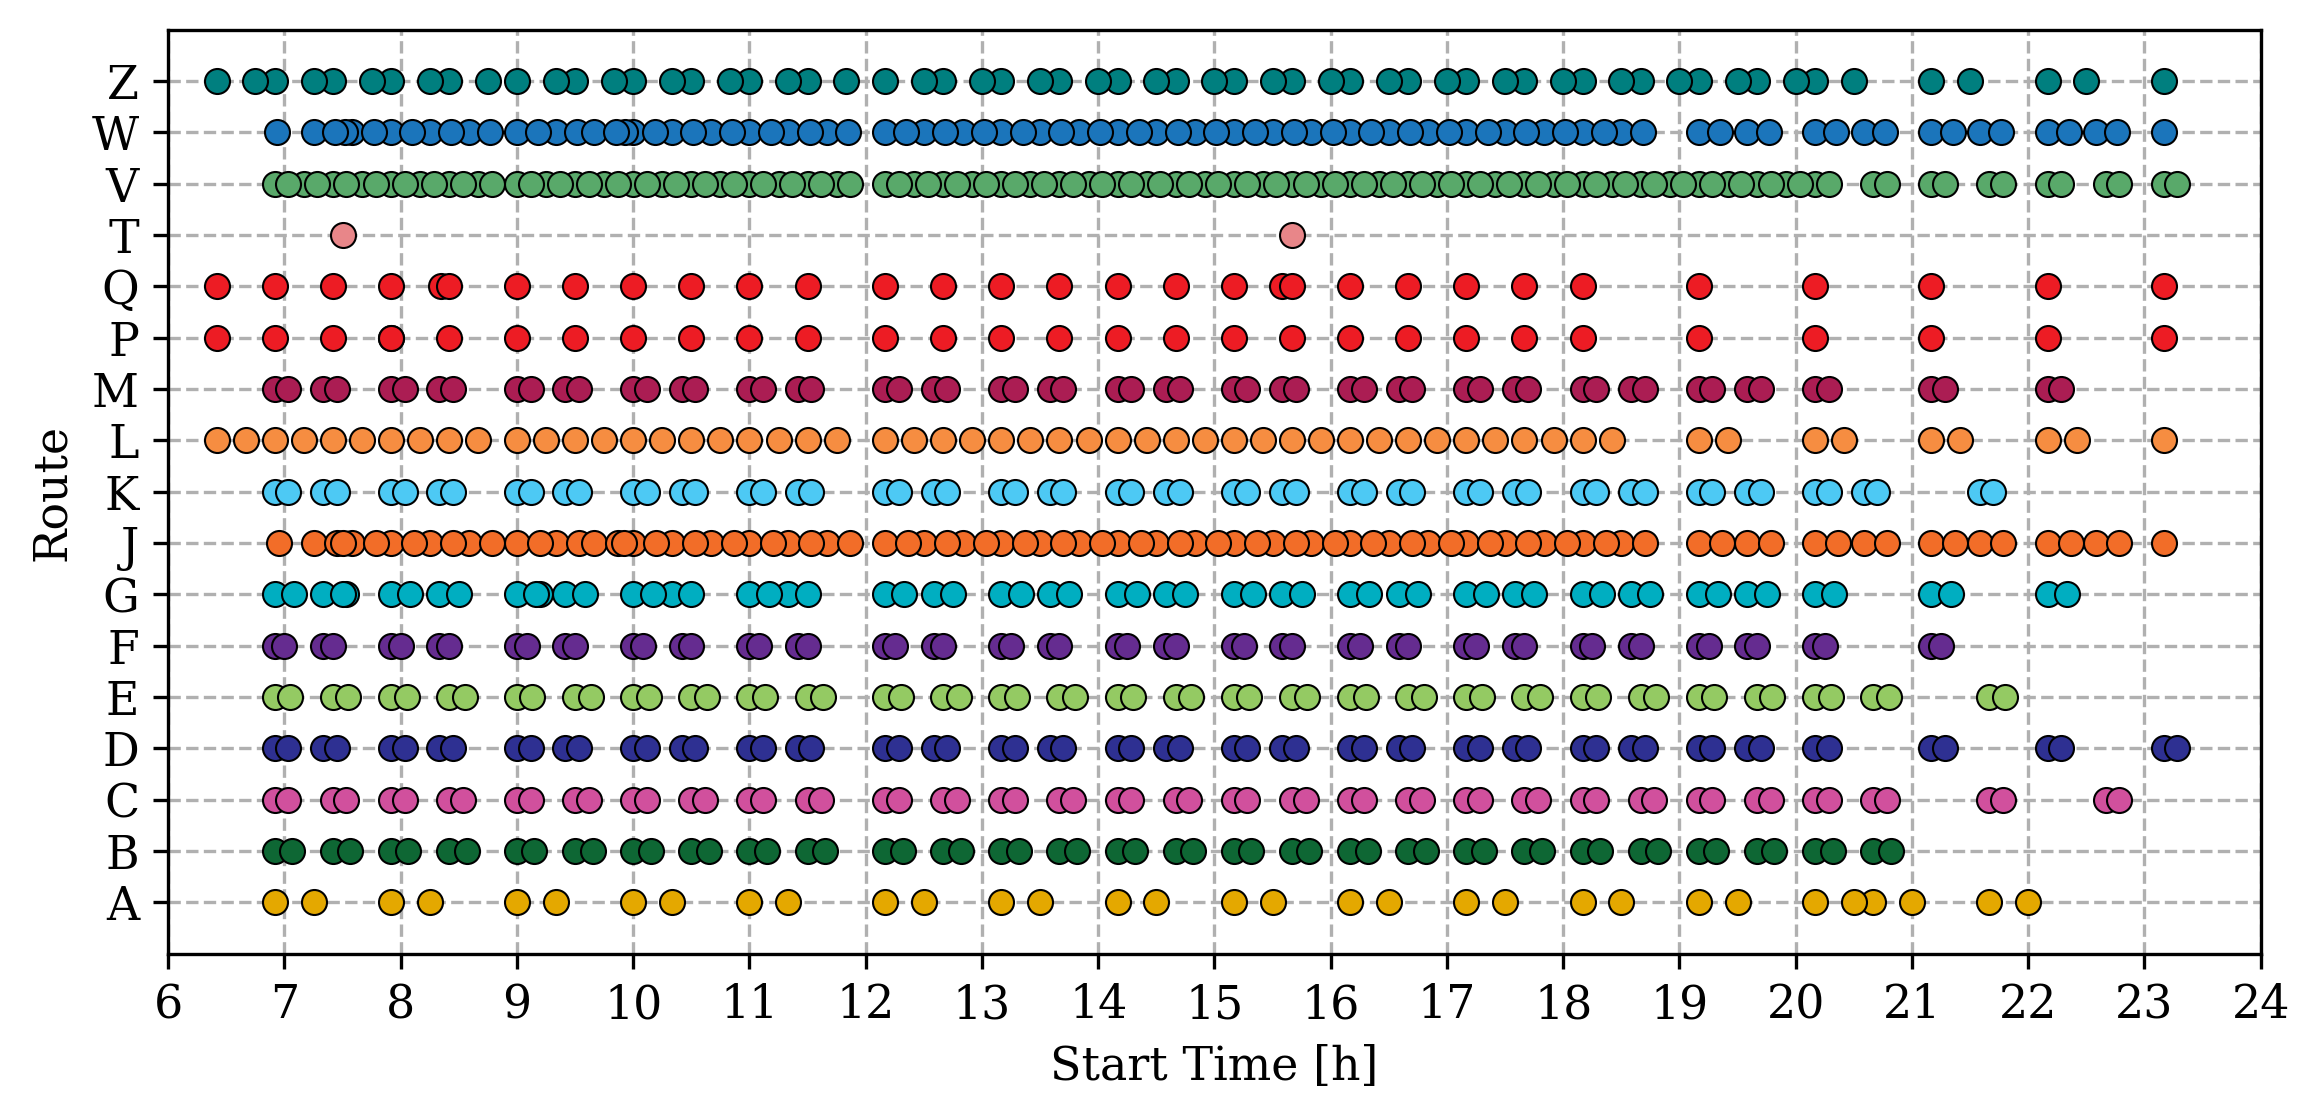
\includegraphics[width = \figurewidth]{figs/unitrans_trips.png}
	\caption{}
	\label{fig:unitrans_trips}
\end{figure}

The vehicle and supply equipment models used in this case study are inexact and meant to be representative rather than specific. Actual costs will vary meaningfully by operator. Parameters given are informed by technical reports of real world implementations \cite{Jeffers_2021_OSTI, Eudy_2021_OSTI, Post_2023_OSTI} and journal papers \cite{Rout_2022_H, Chen_2024_S, Sistig_2025_SMT}.

For these examples five different vehicle types are considered. These include three different \glspl{ev}, a \gls{srbev}, \gls{mrbev}, and a \gls{lrbev}, a \gls{fcev}, and a diesel \gls{icev}. The bus models are described in Table \ref{tab:vehicle_types}. The technical parameters are based on NewFlyer models \cite{CHVIP_2025} and the costs are based on APTA purchase prices data \cite{APTA_2025}.

\begin{table}[H]
	\centering
	\caption{}
	\label{tab:vehicle_types}
	\begin{tabular}{|C{.2\linewidth}|C{.2\linewidth}|C{.2\linewidth}|C{.2\linewidth}|C{.2\linewidth}|}
		\hline Vehicle Type & Capacity [kWh] & Maximum Supply Rate [kW] & Consumption [kWh / km] & Unit Cost [USD] \\
		\hline \gls{srbev} & 440 & 350 & 1.25 & 800,000 \\
		\hline \gls{mrbev} & 550 & 350 & 1.3 & 1,000,000 \\
		\hline \gls{lrbev} & 660 & 350 & 1.35 & 1,200,000 \\
		\hline \gls{fcev} & 1,277.5 & 10,950 & 2.81 & 1,600,000 \\
		\hline \gls{icev} & 5,180 & 88,800 & 2.23 & 280,000 \\
		\hline
	\end{tabular}
\end{table}

The four different supply port types in Table \ref{tab:port_types} are also considered. These are AC chargers, DC chargers, Liquefied Hydrogen pumps, and Diesel pumps. The technical and cost parameters are based on transit operator reports. Emissions values are taken from US EPA equivalencies. Electric emissions use the California power grid intensity. H2 production and liquefaction are assumed to be grid powered and thus the emissions intensity is that of the California power grid multiplied by a constant reflecting the energy overhead required. Although the difference in emissions intensity appears small between the energy types, actual emissions scale with energy used and the \glspl{ev} have much lower energy consumption values leading to much lower gross emissions per km driven.

\begin{table}[H]
\centering
\caption{}
\label{tab:port_types}
\begin{tabular}{|C{.2\linewidth}|C{.2\linewidth}|C{.2\linewidth}|C{.2\linewidth}|C{.2\linewidth}|}
	\hline port Type & Maximum Supply Rate [kW] & Emissions [gC02 / kWh] & Unit Cost [USD] & Fixed Cost [USD]\\
	\hline AC-PLUG & 19 & 225.6 & 5,000 & 10,000\\
	\hline DC-PLUG & 150 & 225.6 & 30,000 & 50,000 \\
	\hline LH2-PUMP & 10,950 & 322.3 &  100,000 & 250,000 \\
	\hline DIESEL-PUMP & 88,800 & 275.1 & 30,000 & 50,000 \\
	\hline
\end{tabular}
\end{table}

The single depot that Unitrans operates out of is space limited both in terms of overall parking and in terms port capacity. In this example the parking spaces for the fleet are limited to 60 which also limits the fleet size to 60 buses. There are 10 total available spaces for dedicated charging/fueling. This limits the total number of DC charging stations, hydrogen pumps, and diesel pumps to 10. Because AC chargers are small in footprint one can be added for each parking spot.

In this example the objectives are capital cost and daily cost. Capital Cost includes the costs of purchasing vehicles and supply equipment. Vehicle cost is based only on unit cost while supply equipment cost includes both the unit cost per port and a fixed cost paid before any ports of a given type can be installed. Daily cost encompasses operational costs, energy costs, and labor costs. Operational costs are assumed to scale with distance driven, energy costs are assumed to scale with energy consumed, and labor costs are assumed to scale with operating time (a fixed hourly rate of 20 USD per hour is used for drivers).

Given the vehicle and port options and the weekday schedule, an optimization was run with the following hyper-parameters: population size $M = 150$, generations range $N^- = 300$, $N^+ = 500$, probability of crossover $\phi_c = 0.5$, and probability of mutation $\phi_m = 0.05$. Iteration was terminated after 344 generations when zero children were selected for 5 consecutive generations. The evolution of the population over time is displayed in Figure \ref{fig:evolution_unitrans}.

\begin{figure}[H]
	\centering
	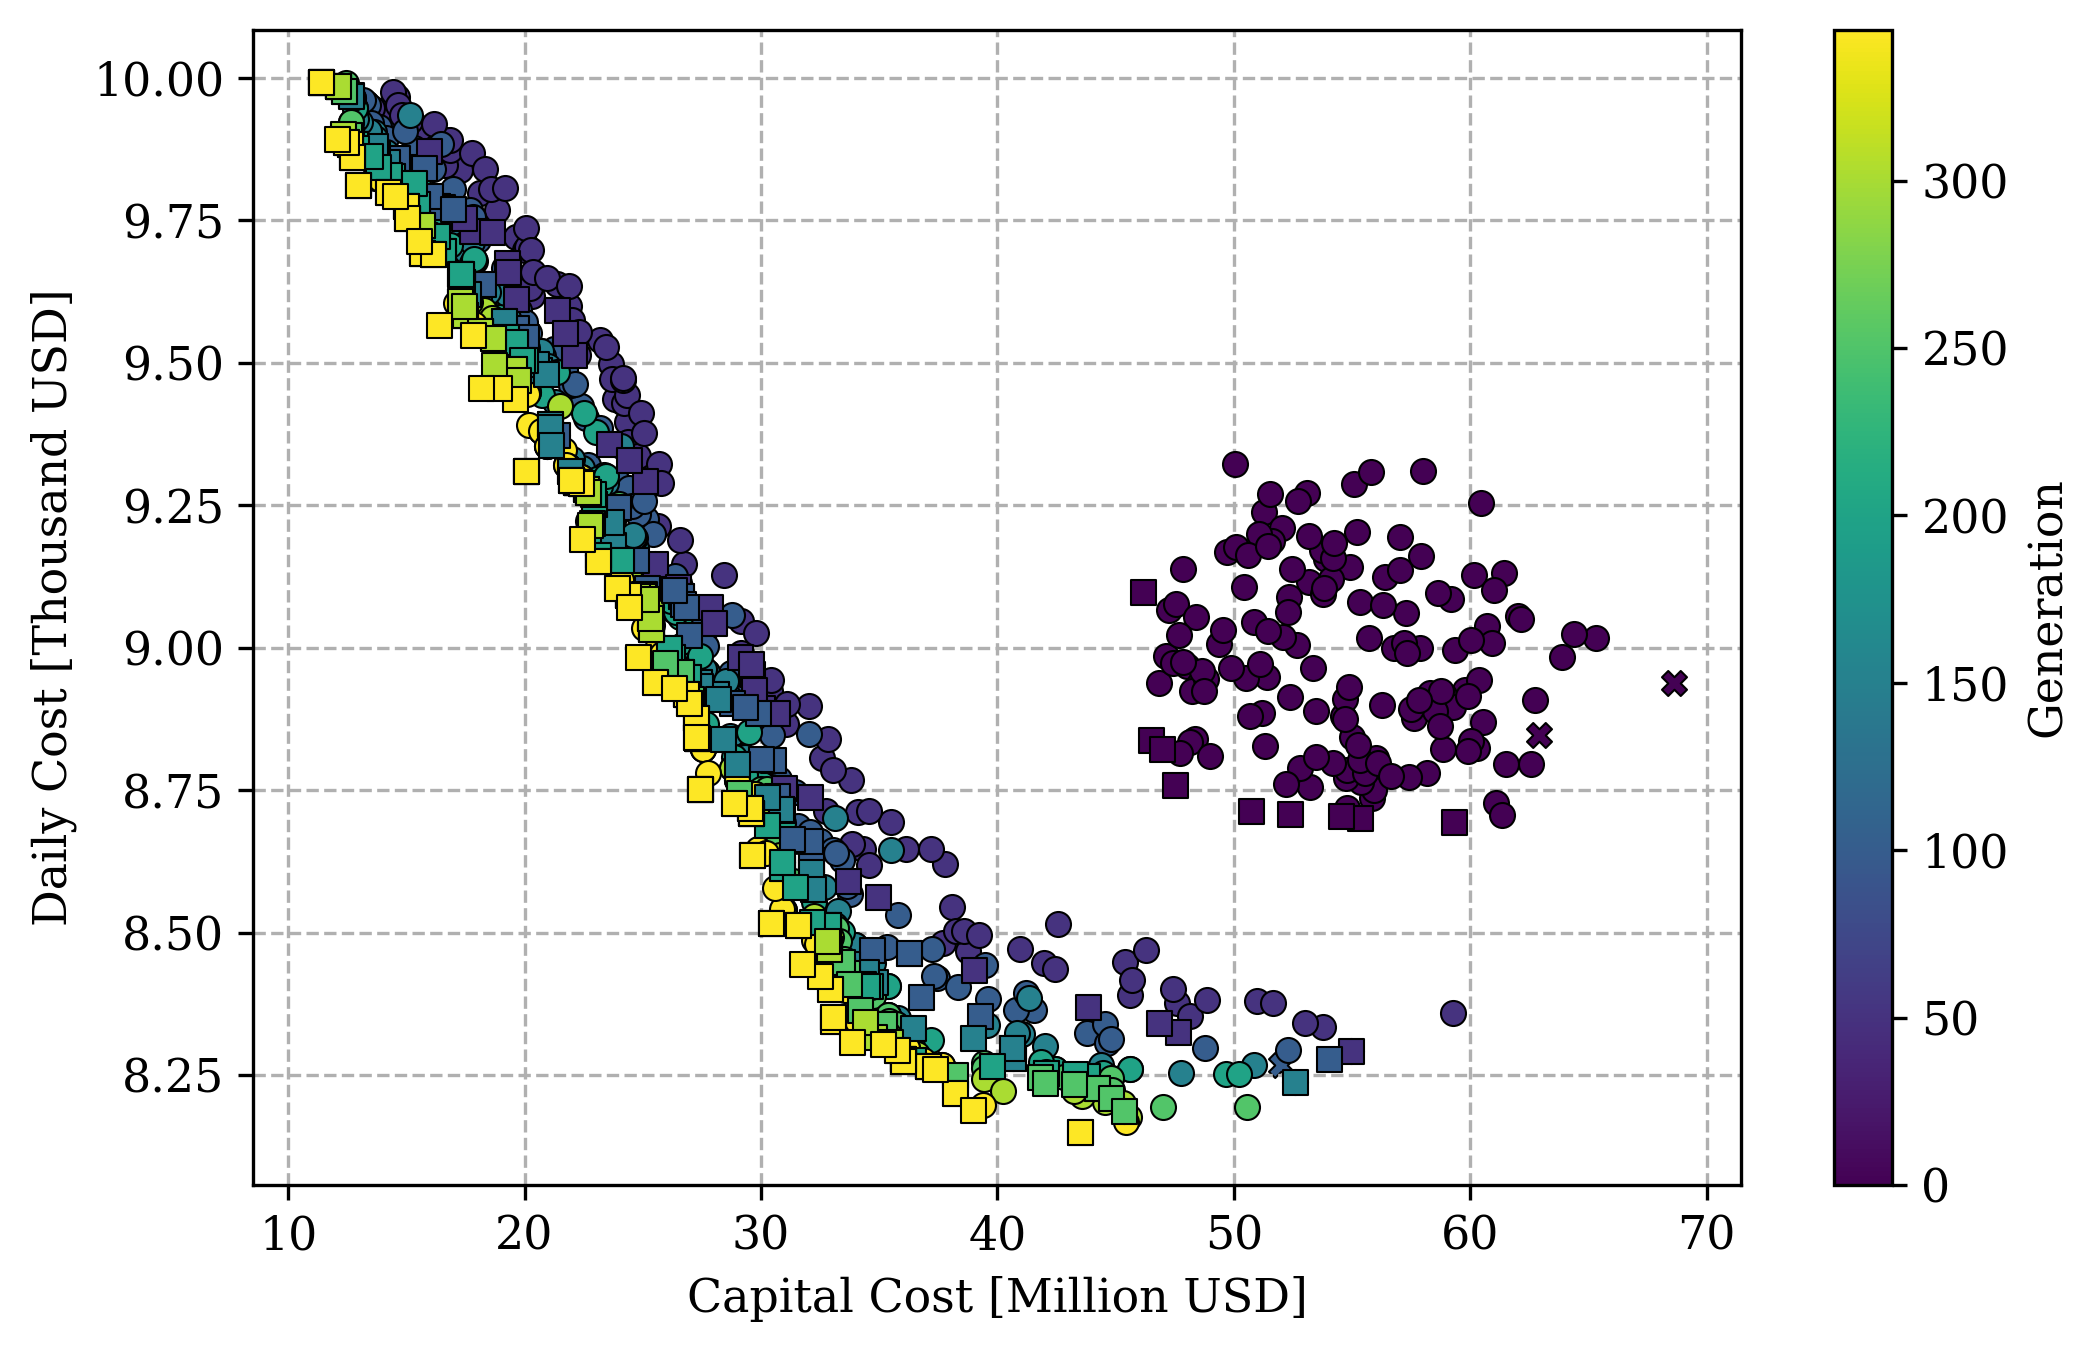
\includegraphics[width = \linewidth]{figs/evolution_unitrans.png}
	\caption{}
	\label{fig:evolution_unitrans}
\end{figure}

As can be seen, the pace of evolution is rapid initially but becomes slow after about 100 iterations. Possibly, different hyper-parameter settings could result in quicker convergence at the cost of increasing the likelihood if premature termination. The final Pareto front and fleet compositions and sizes are shown in Figures \ref{fig:unitrans_baseline_scatter_pie} and \ref{fig:unitrans_baseline_stacked_bar}.

\begin{figure}[H]
	\centering
	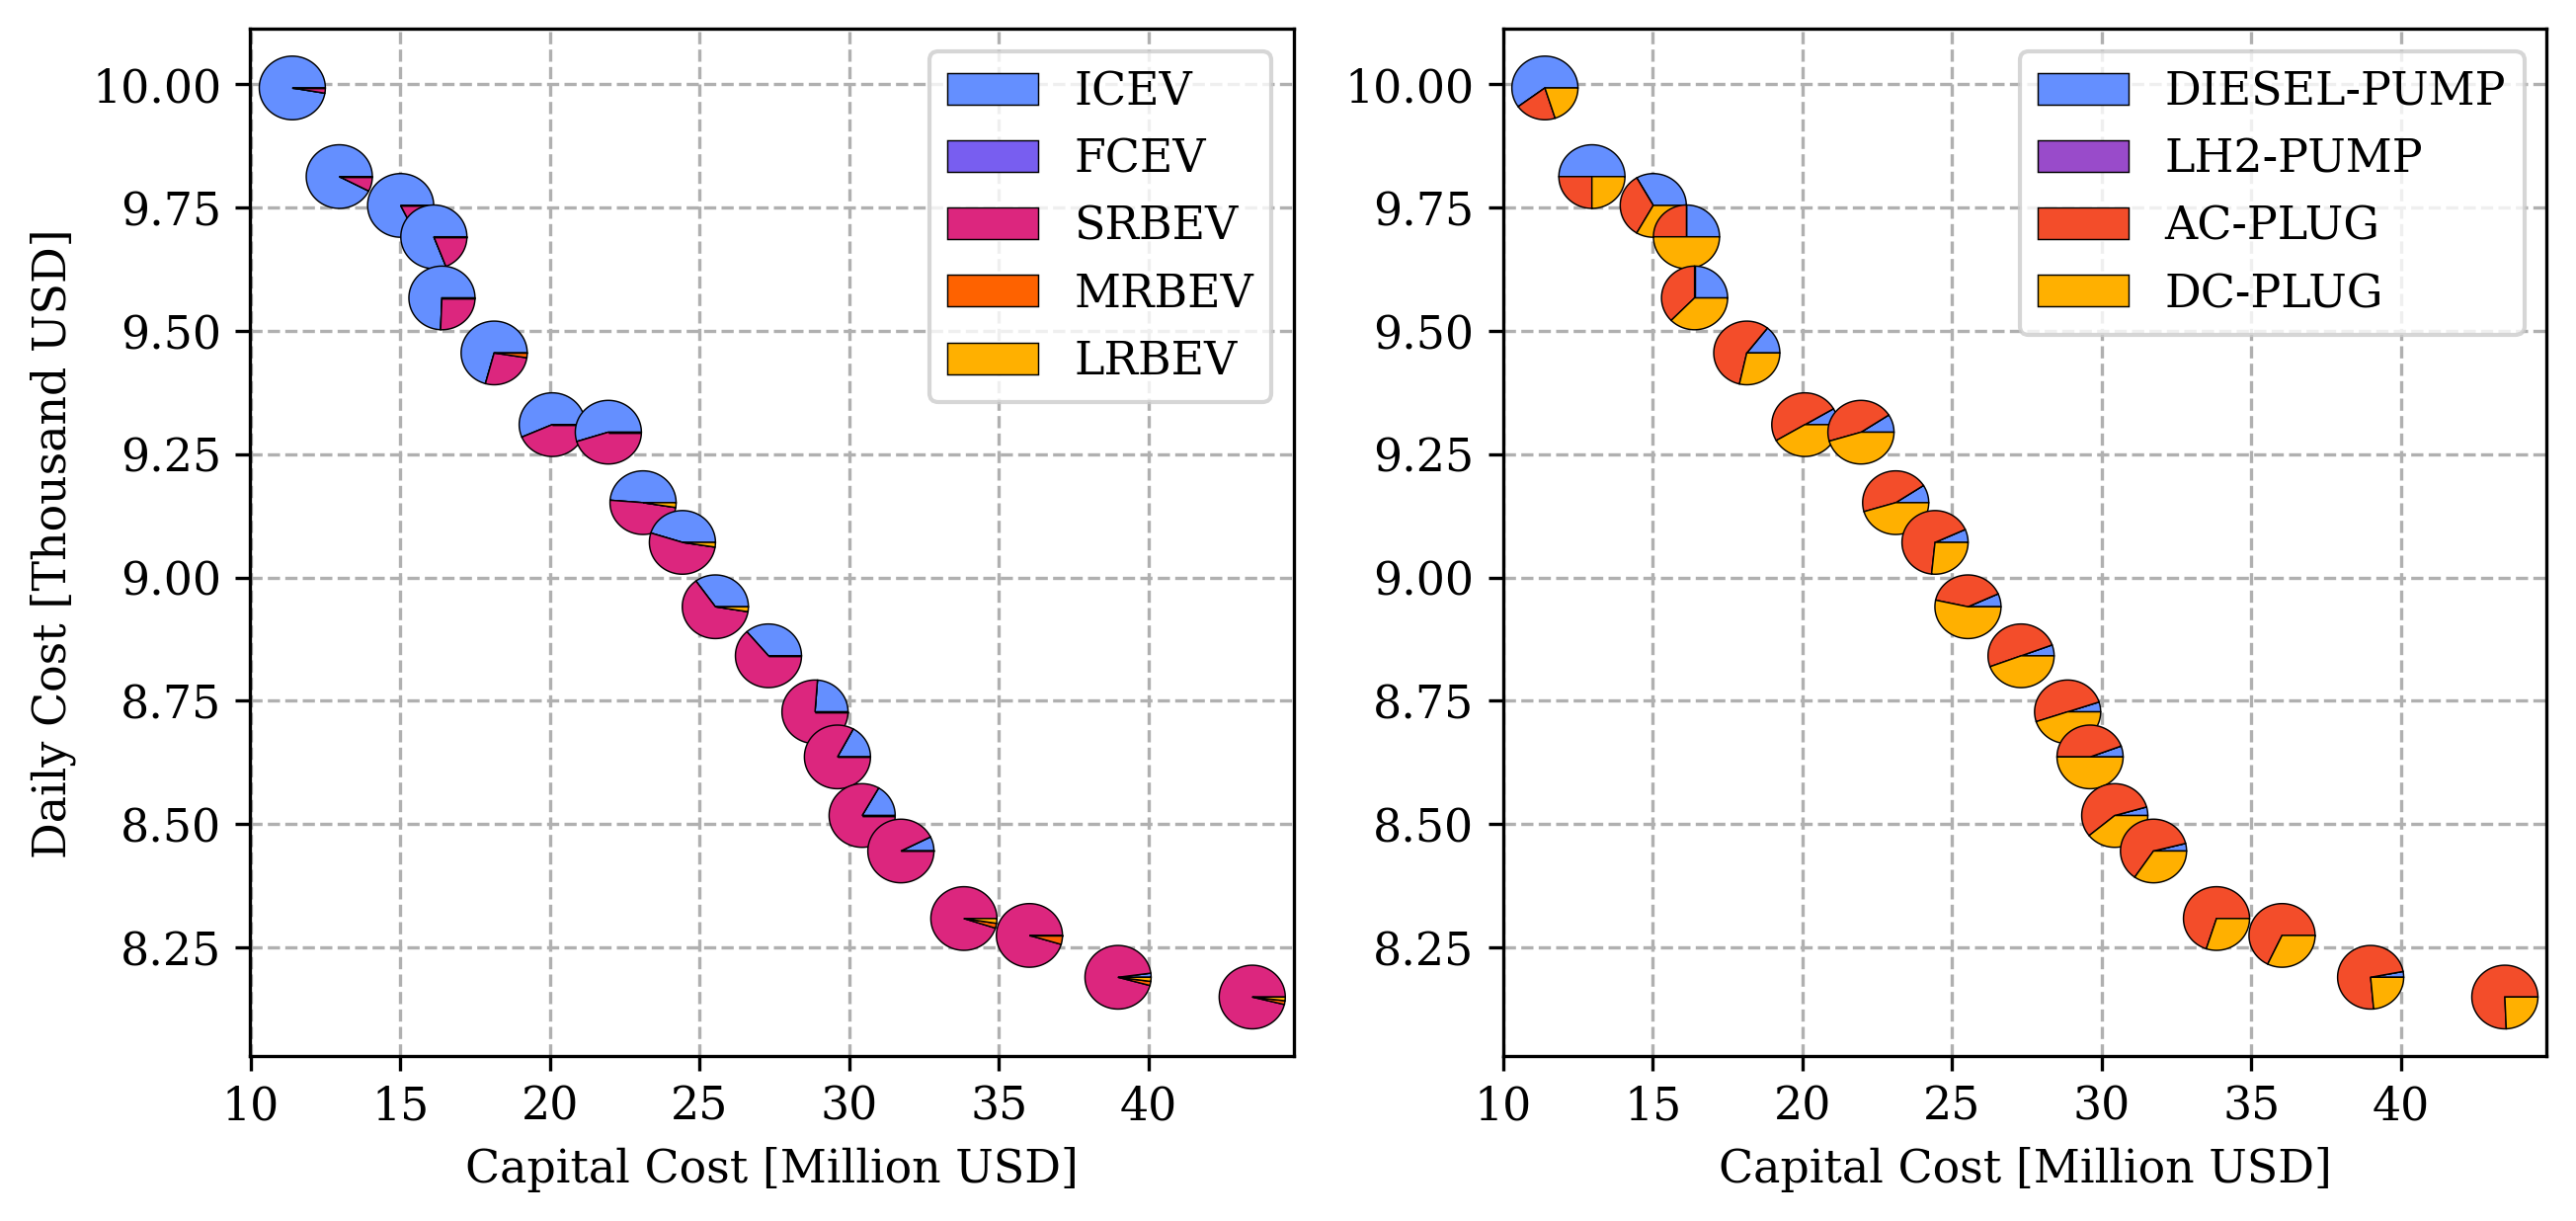
\includegraphics[width = \linewidth]{figs/unitrans_baseline_scatter_pie.png}
	\caption{}
	\label{fig:unitrans_baseline_scatter_pie}
\end{figure}

\begin{figure}[H]
	\centering
	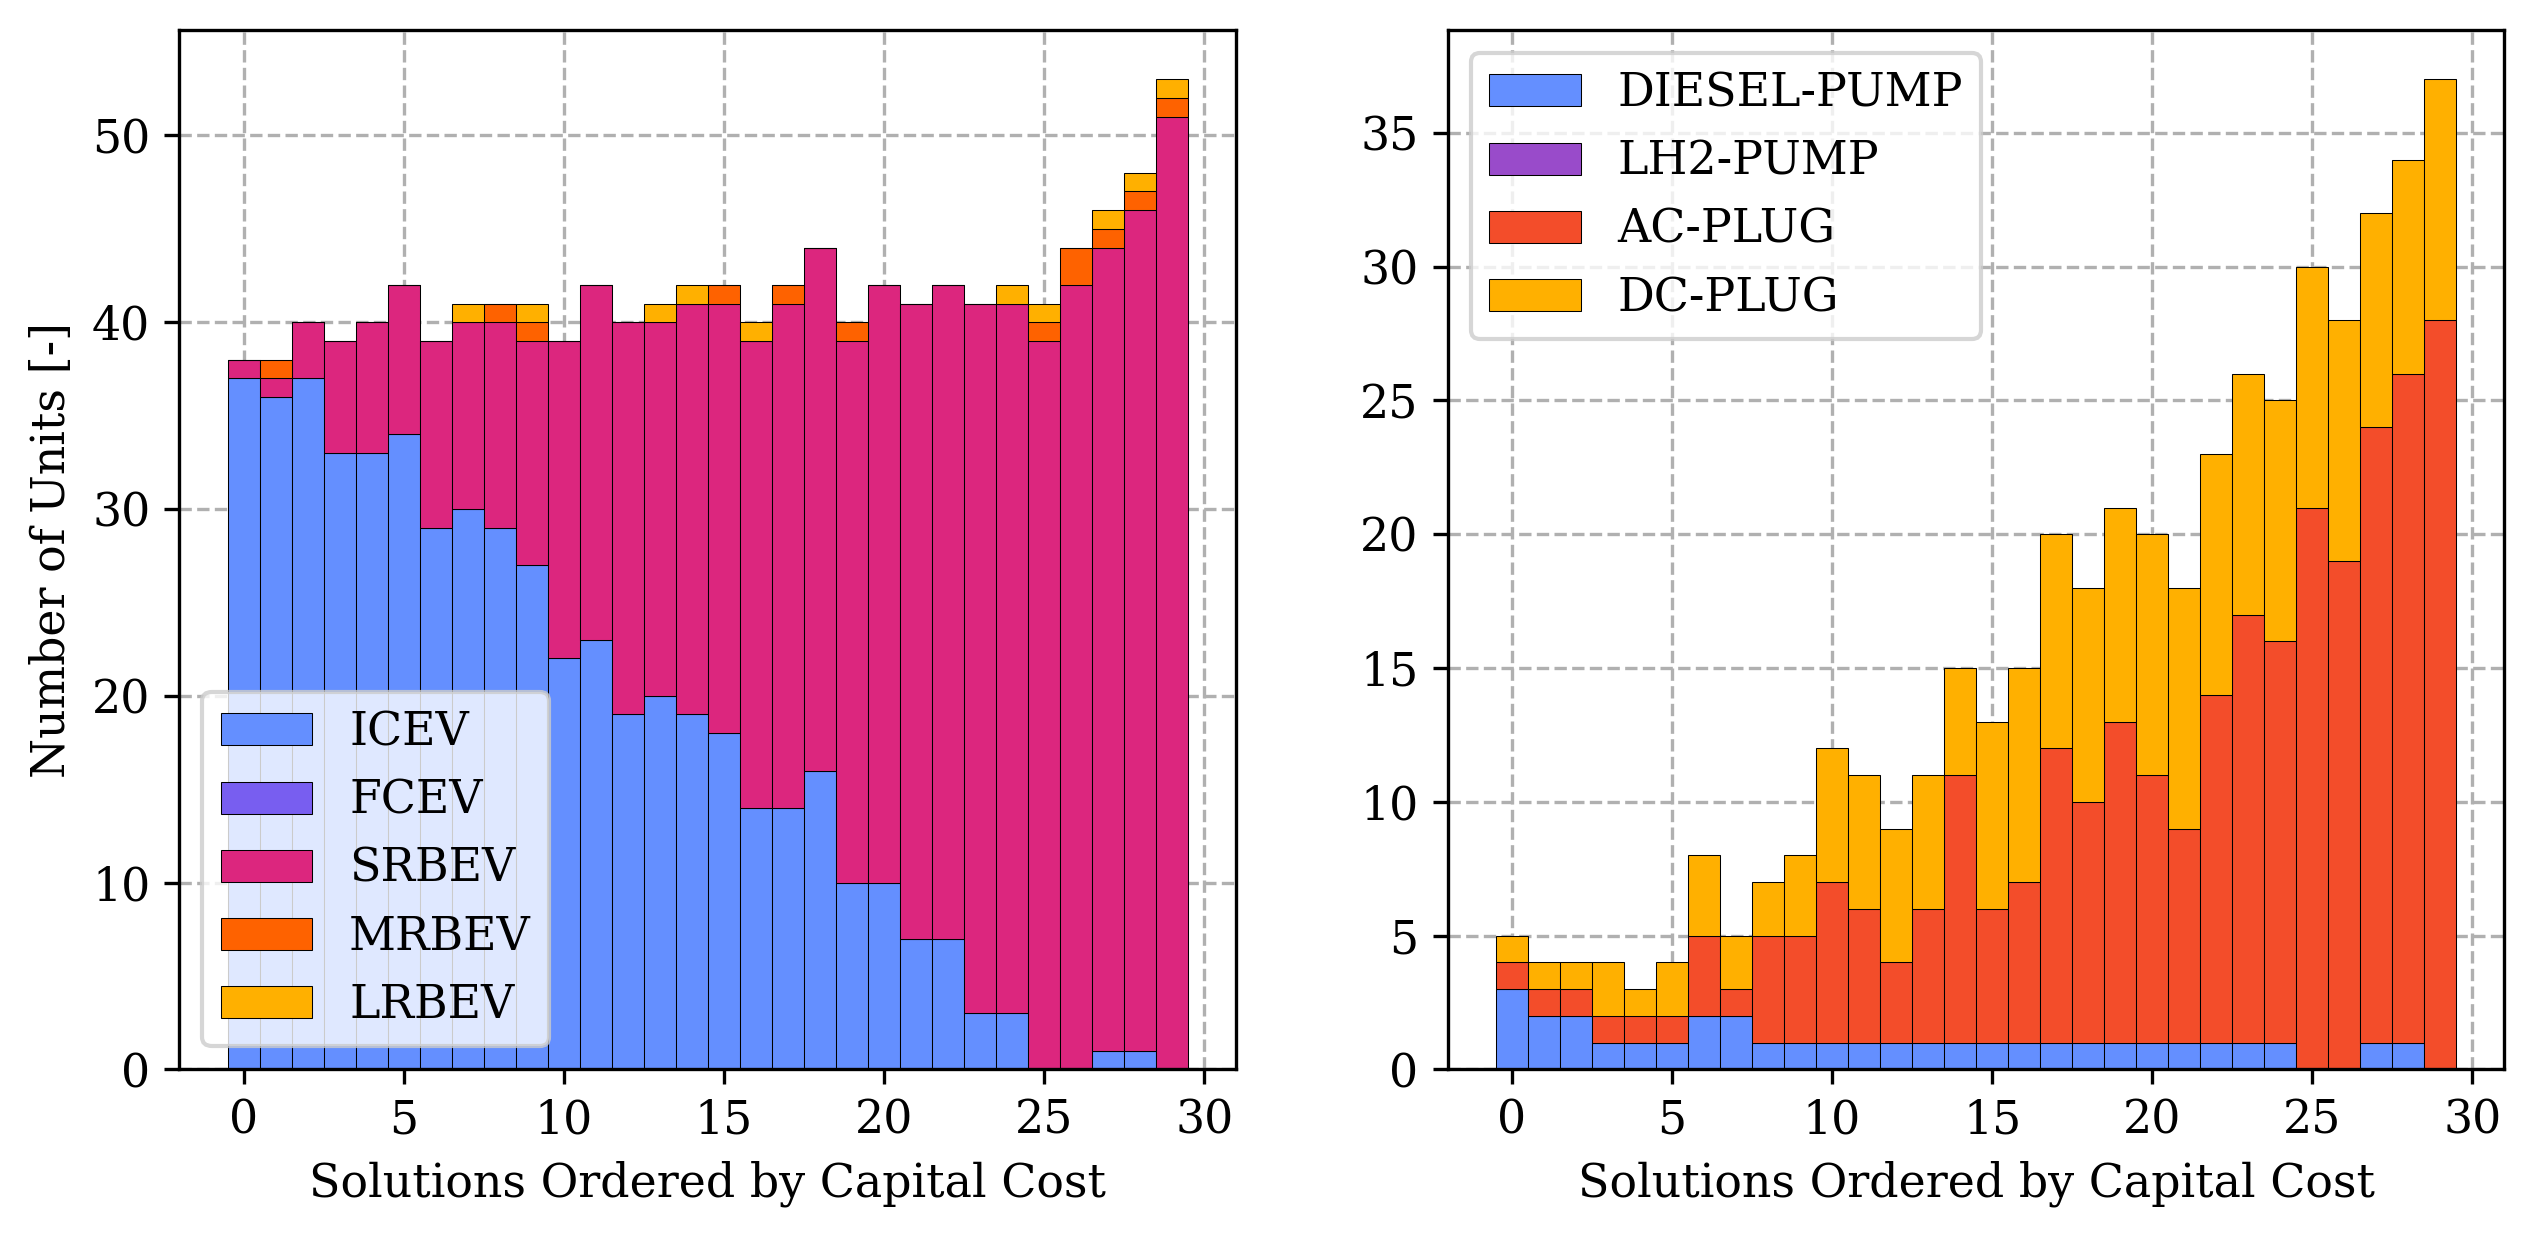
\includegraphics[width = \linewidth]{figs/unitrans_baseline_stacked_bar.png}
	\caption{}
	\label{fig:unitrans_baseline_stacked_bar}
\end{figure}

Figure \ref{fig:unitrans_baseline_scatter_pie} shows the Pareto front as a scatter plot of pie charts for both vehicles and supply infrastructure. The composition of the fleet is reflected in the slices of the pie charts. As can be seen, solutions which present low capital costs and high daily costs are dominantly composed of Diesel \glspl{icev}. On the opposite end high capital cost, low daily cost solutions are dominantly composed of \glspl{srbev}. Options such as the \gls{mrbev}, \gls{lrbev}, and \gls{fcev} are minimally present. This is likely due to the small geographic area Unitrans services and the frequency of trips. Because the vehicle fleets at the high daily cost end of the front are \gls{icev} dominated, there is little reason to build other infrastructure. Additionally because \gls{icev} fueling is rapid, there is no reason to build a large number of pumps. Moving towards the high capital cost end of the front, \gls{bev} charging infrastructure becomes more prevalent. Initially this is largely DC chargers due and eventually becomes mostly AC chargers due to the constraint on the number of DC chargers that can be built. Vehicle fleet sizes remain roughly constant at around 40 vehicles throughout the front until the high-capita-cost extreme. The actual Unitrans fleet contains around 50 vehicles but this number accounts for maintenance cycles which are not modeled in this paper.

\subsection{SFMTA}

The second case study concerns a much larger bus network. \gls{sfmta} operates a bus network which connects locations within the city of San Francisco which is geographically large and densely populated by US standards. A Monday schedule for \gls{sfmta} consists of 8,993 scheduled trips operating from six primary depots. Unlike Unitrans, route terminals are scattered throughout the city. Weekday service runs from 4 AM through midnight and most routes are serviced with high frequency as seen in Figure \ref{fig:sfmta_trips}.

\begin{figure}[H]
	\centering
	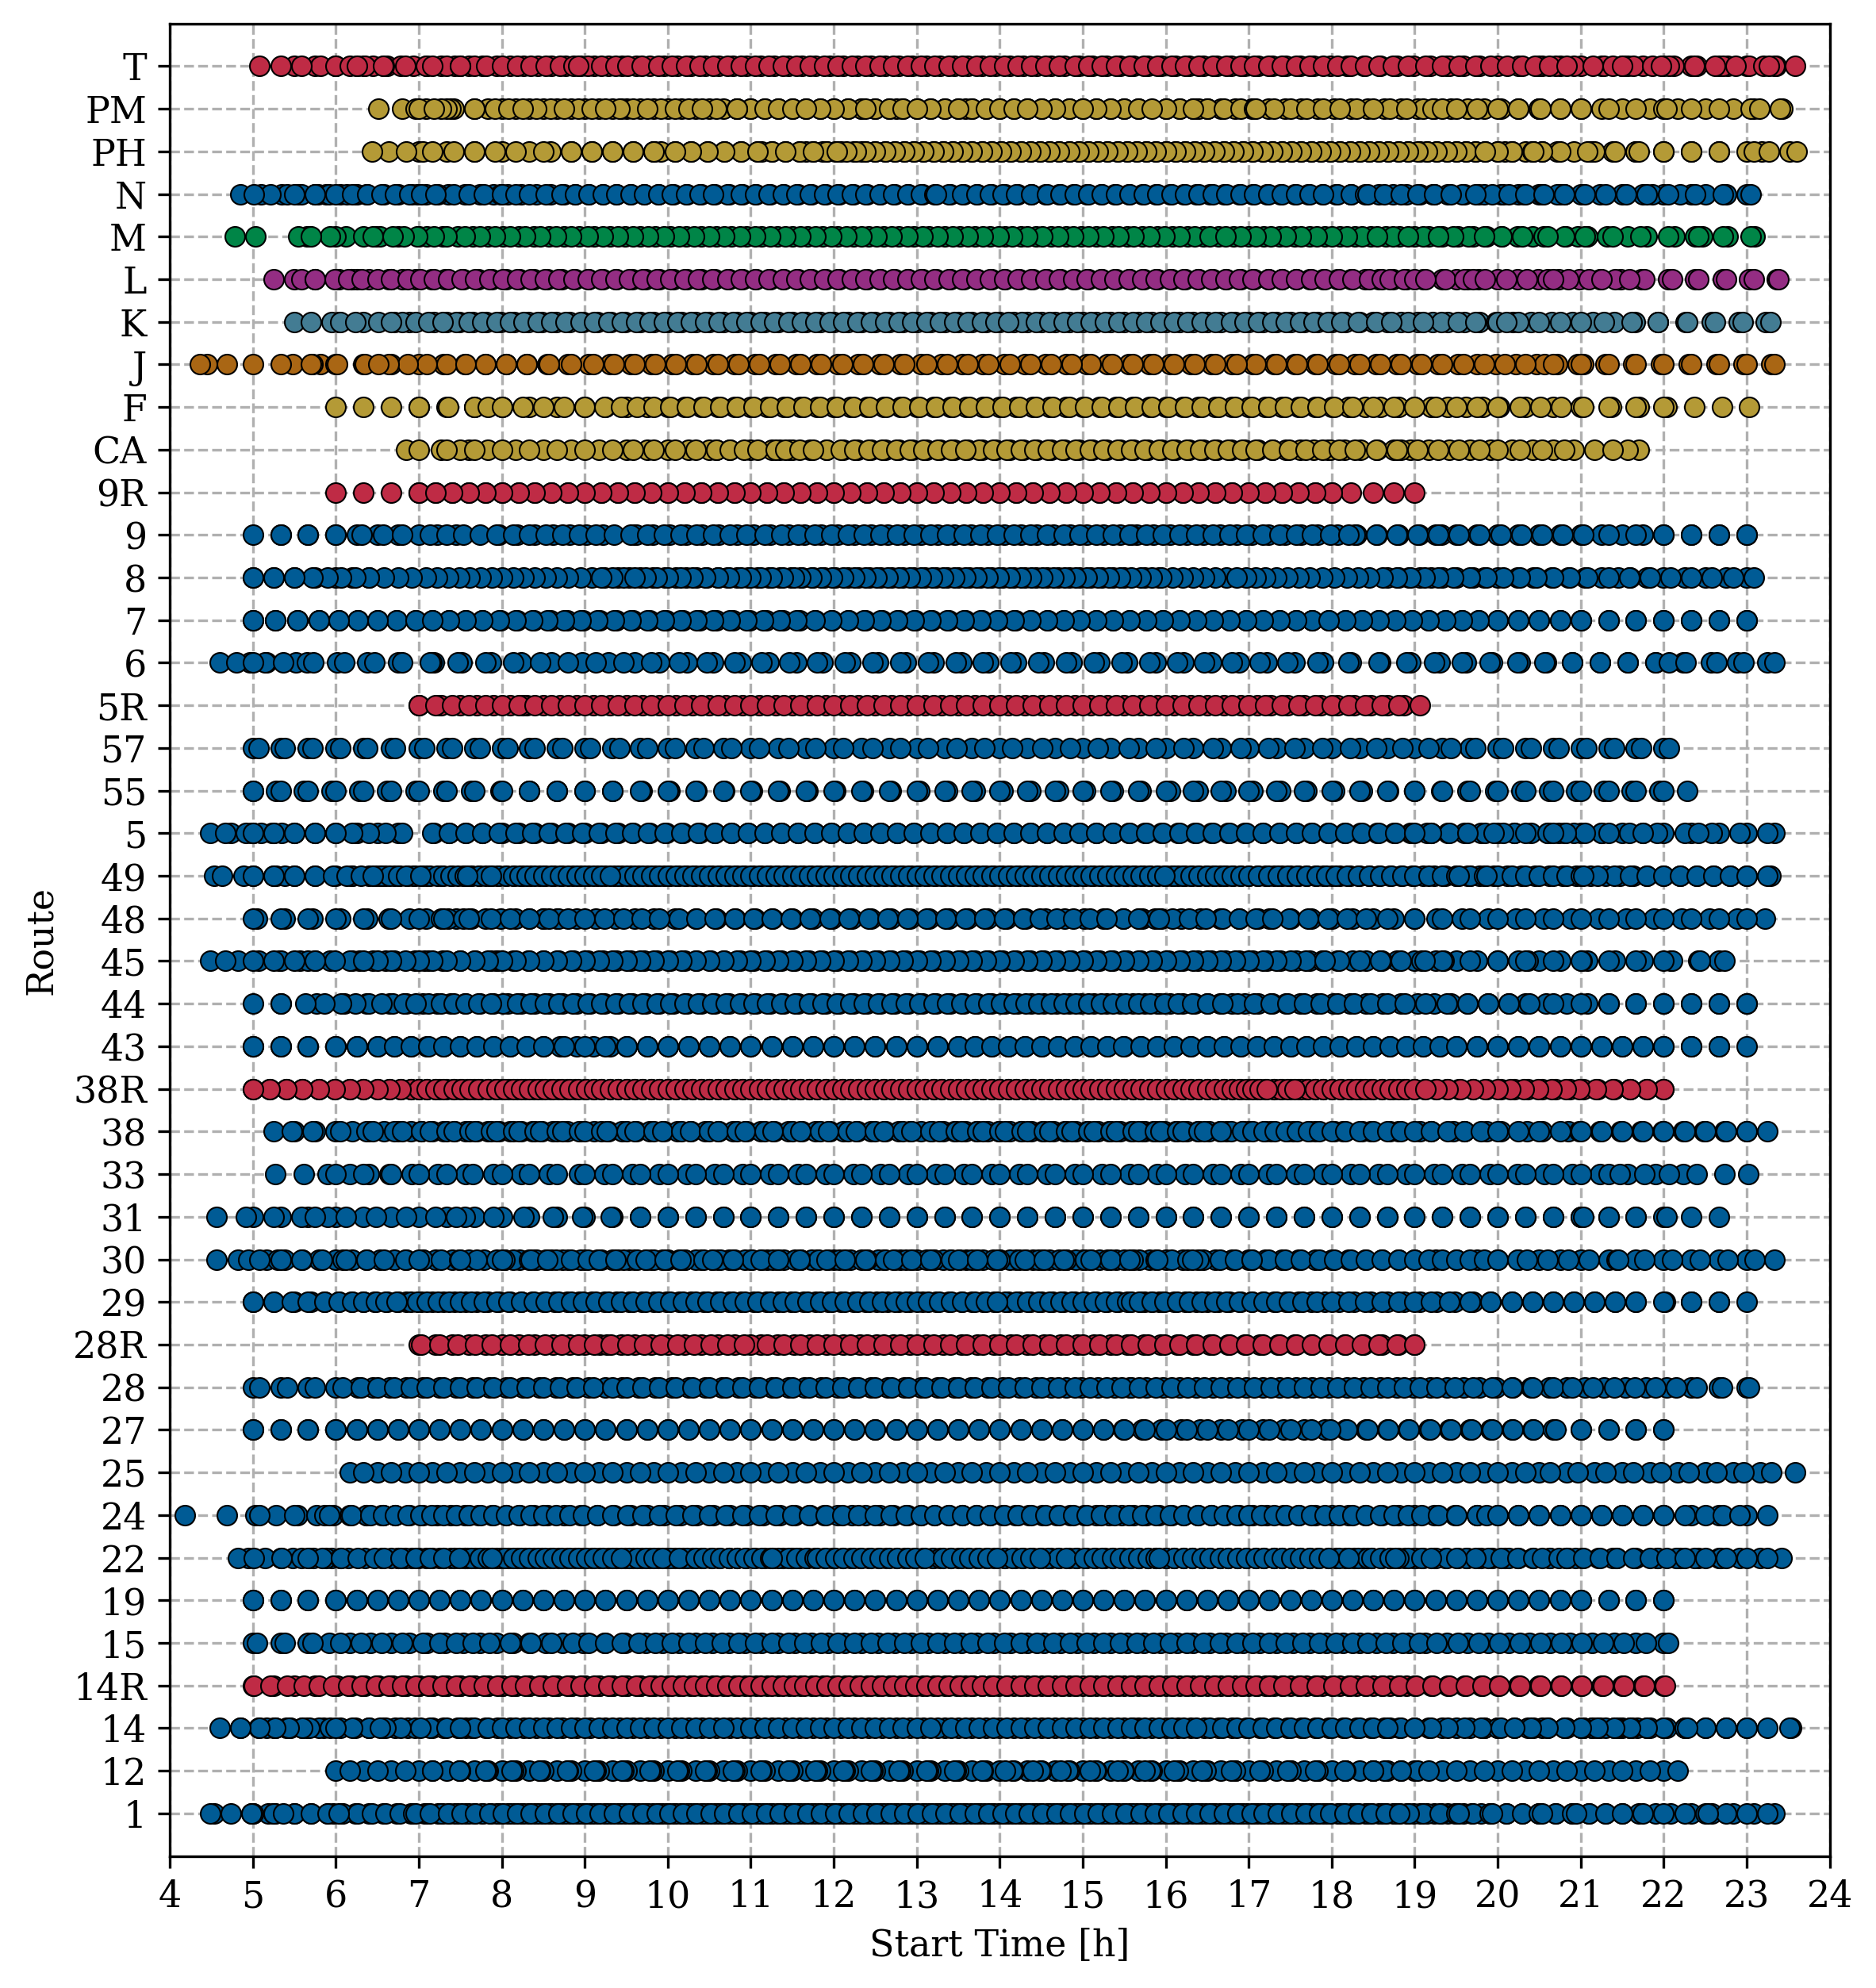
\includegraphics[width = \figurewidth]{figs/sfmta_trips.png}
	\caption{}
	\label{fig:sfmta_trips}
\end{figure}

Using the same vehicle and port options as with Unitrans, an optimization was run with the following hyper-parameters: population size $M = 200$, generations range $N^- = 500$, $N^+ = 1000$, probability of crossover $\phi_c = 0.5$, and probability of mutation $\phi_m = 0.15$. Iteration was terminated after 759 generations when zero children were selected for 5 consecutive generations. The evolution of the population over time is displayed in Figure \ref{fig:evolution_sfmta}.

\begin{figure}[H]
	\centering
	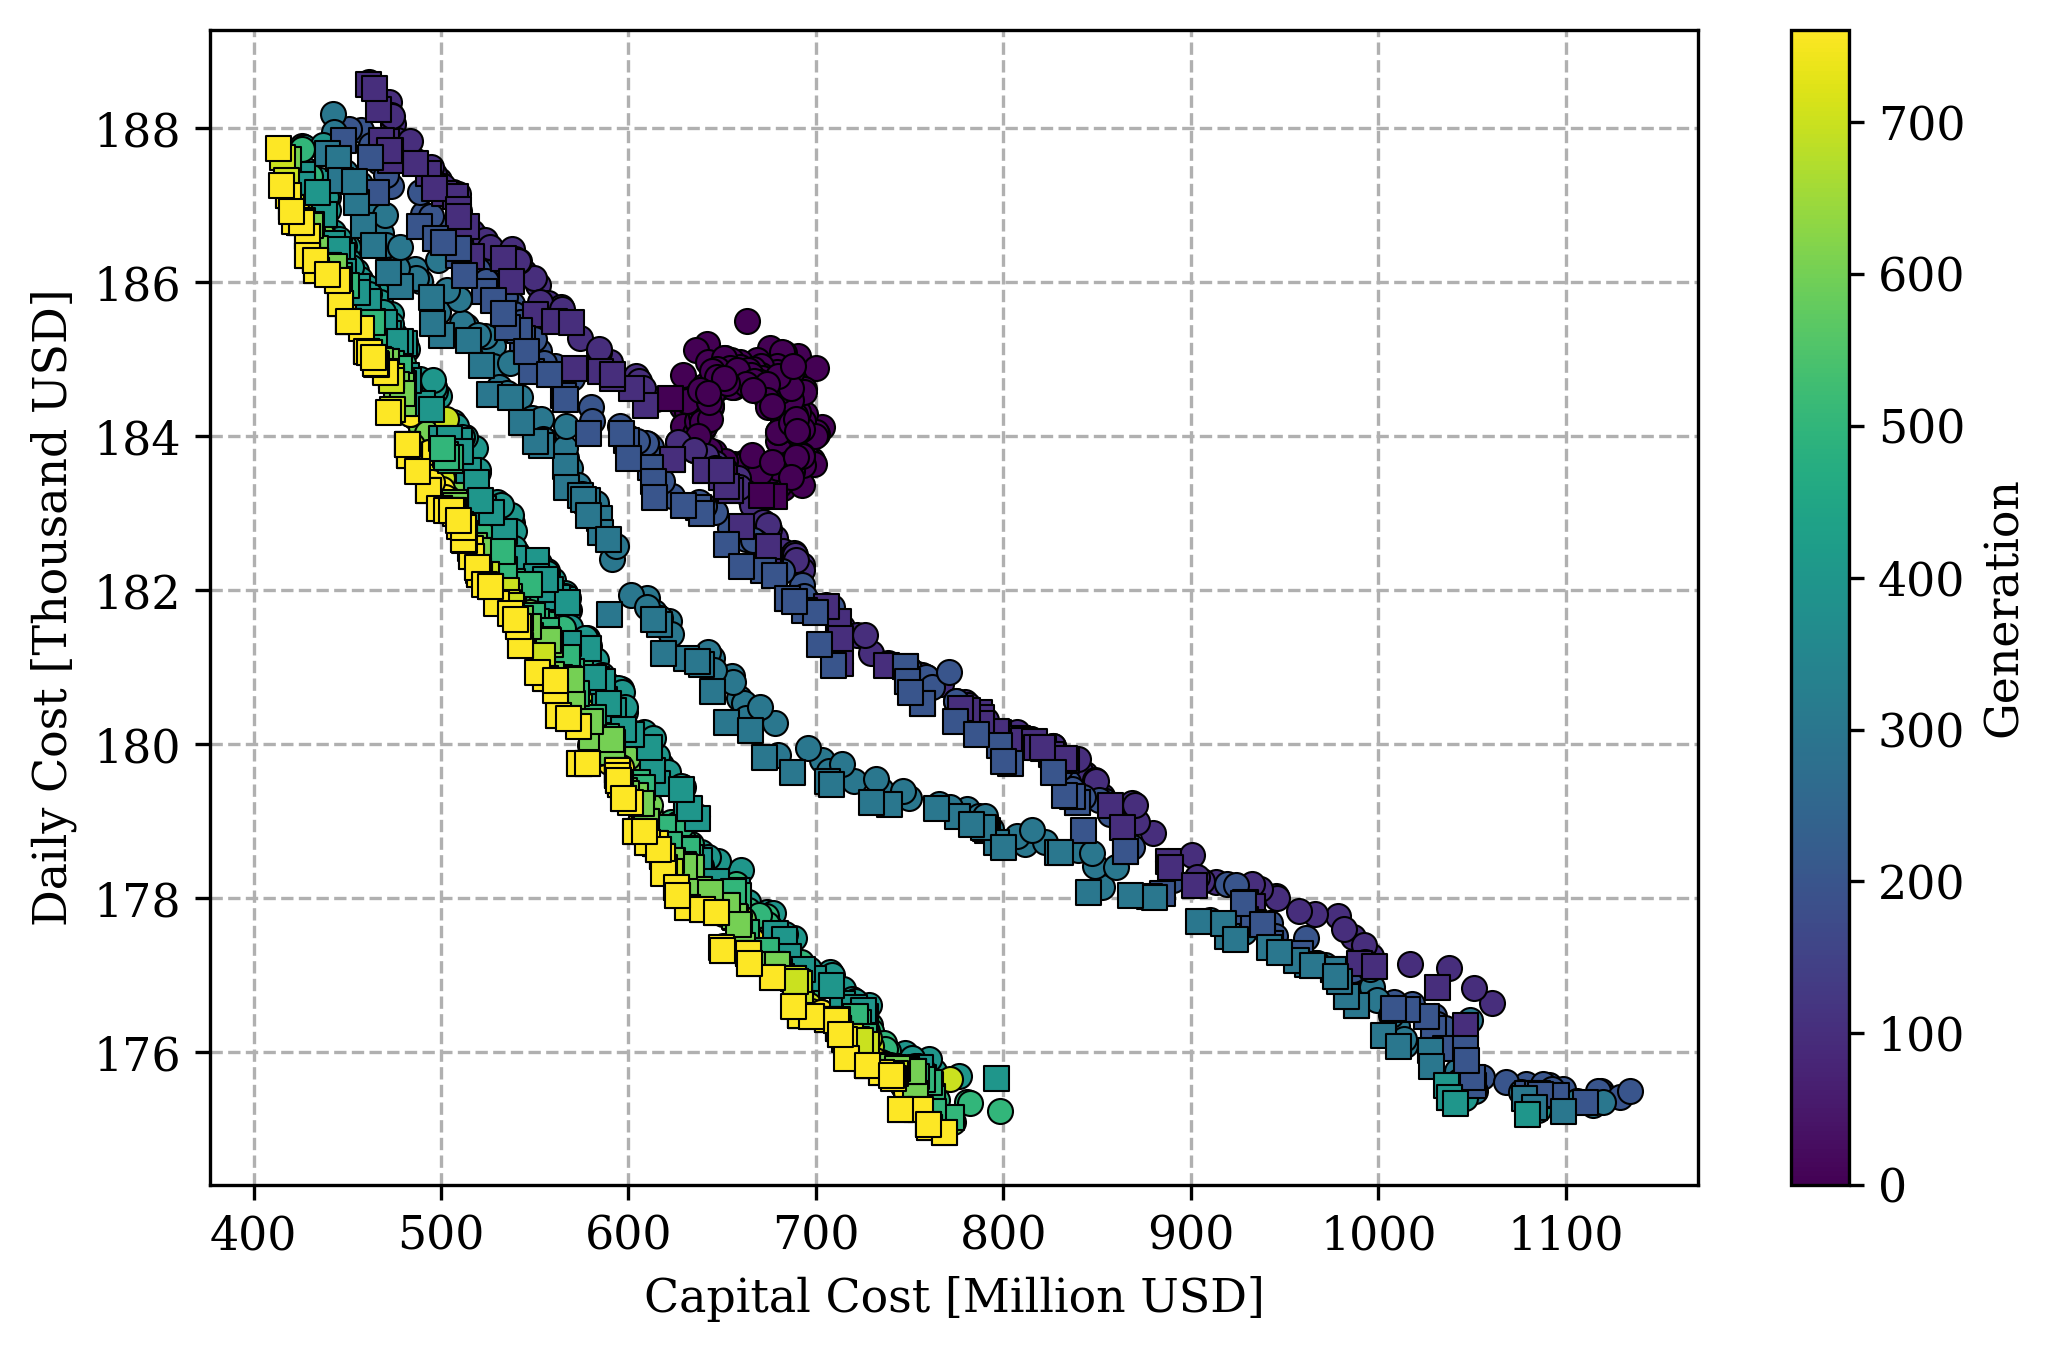
\includegraphics[width = \linewidth]{figs/evolution_sfmta.png}
	\caption{}
	\label{fig:evolution_sfmta}
\end{figure}

Being a much larger network with a exponentially  greater number of possible configurations, the \gls{sfmta} optimization converged slower. Where the Pareto front reached its approximate final shape within 100 generations for Unitrans, this took around 400 generations for \gls{sfmta}. For the \gls{sfmta} case study, a higher mutation probability was used in order to more efficiently explore the design space at the cost of additional randomness. After reaching an approximate final shape, several hundred generations were required before reaching convergence.

The Pareto front for \gls{sfmta} shows a similar but meaningfully different trade-off to that found for Unitrans reflecting differences in routes, schedules, and economies of scale. As seen in Figure \ref{fig:scatter_pie_vehicles_baseline_sfmta}, the Pareto front for \gls{sfmta} contains substantially mixed fleets with non-negligible numbers of \glspl{mrbev} and \glspl{lrbev} alongside the dominant \glspl{icev} and \glspl{srbev}. On the other hand, supply infrastructure is much more uniform in the \gls{sfmta} Pareto front with AC charging dominating DC charging as seen in Figures \ref{fig:scatter_pie_baseline_sfmta} and \ref{fig:stacked_bar_baseline_sfmta}. This is in contrast in the Unitrans Pareto front which contains substantially DC based solutions. The most important differences are the scale of the bus fleets with additional bus purchases playing a smaller role in overall capital budget for \gls{sfmta} than for Unitrans, the time and energy required to travel from route terminals to depots to charge, and lack of depot supply infrastructure constraints. Unitrans operates over a substantially smaller geographic area and all routes terminate close to the depot allowing for buses to easily return to depot to top-up during the day. This strategy is not as viable for \gls{sfmta}.

\begin{figure}[H]
	\centering
	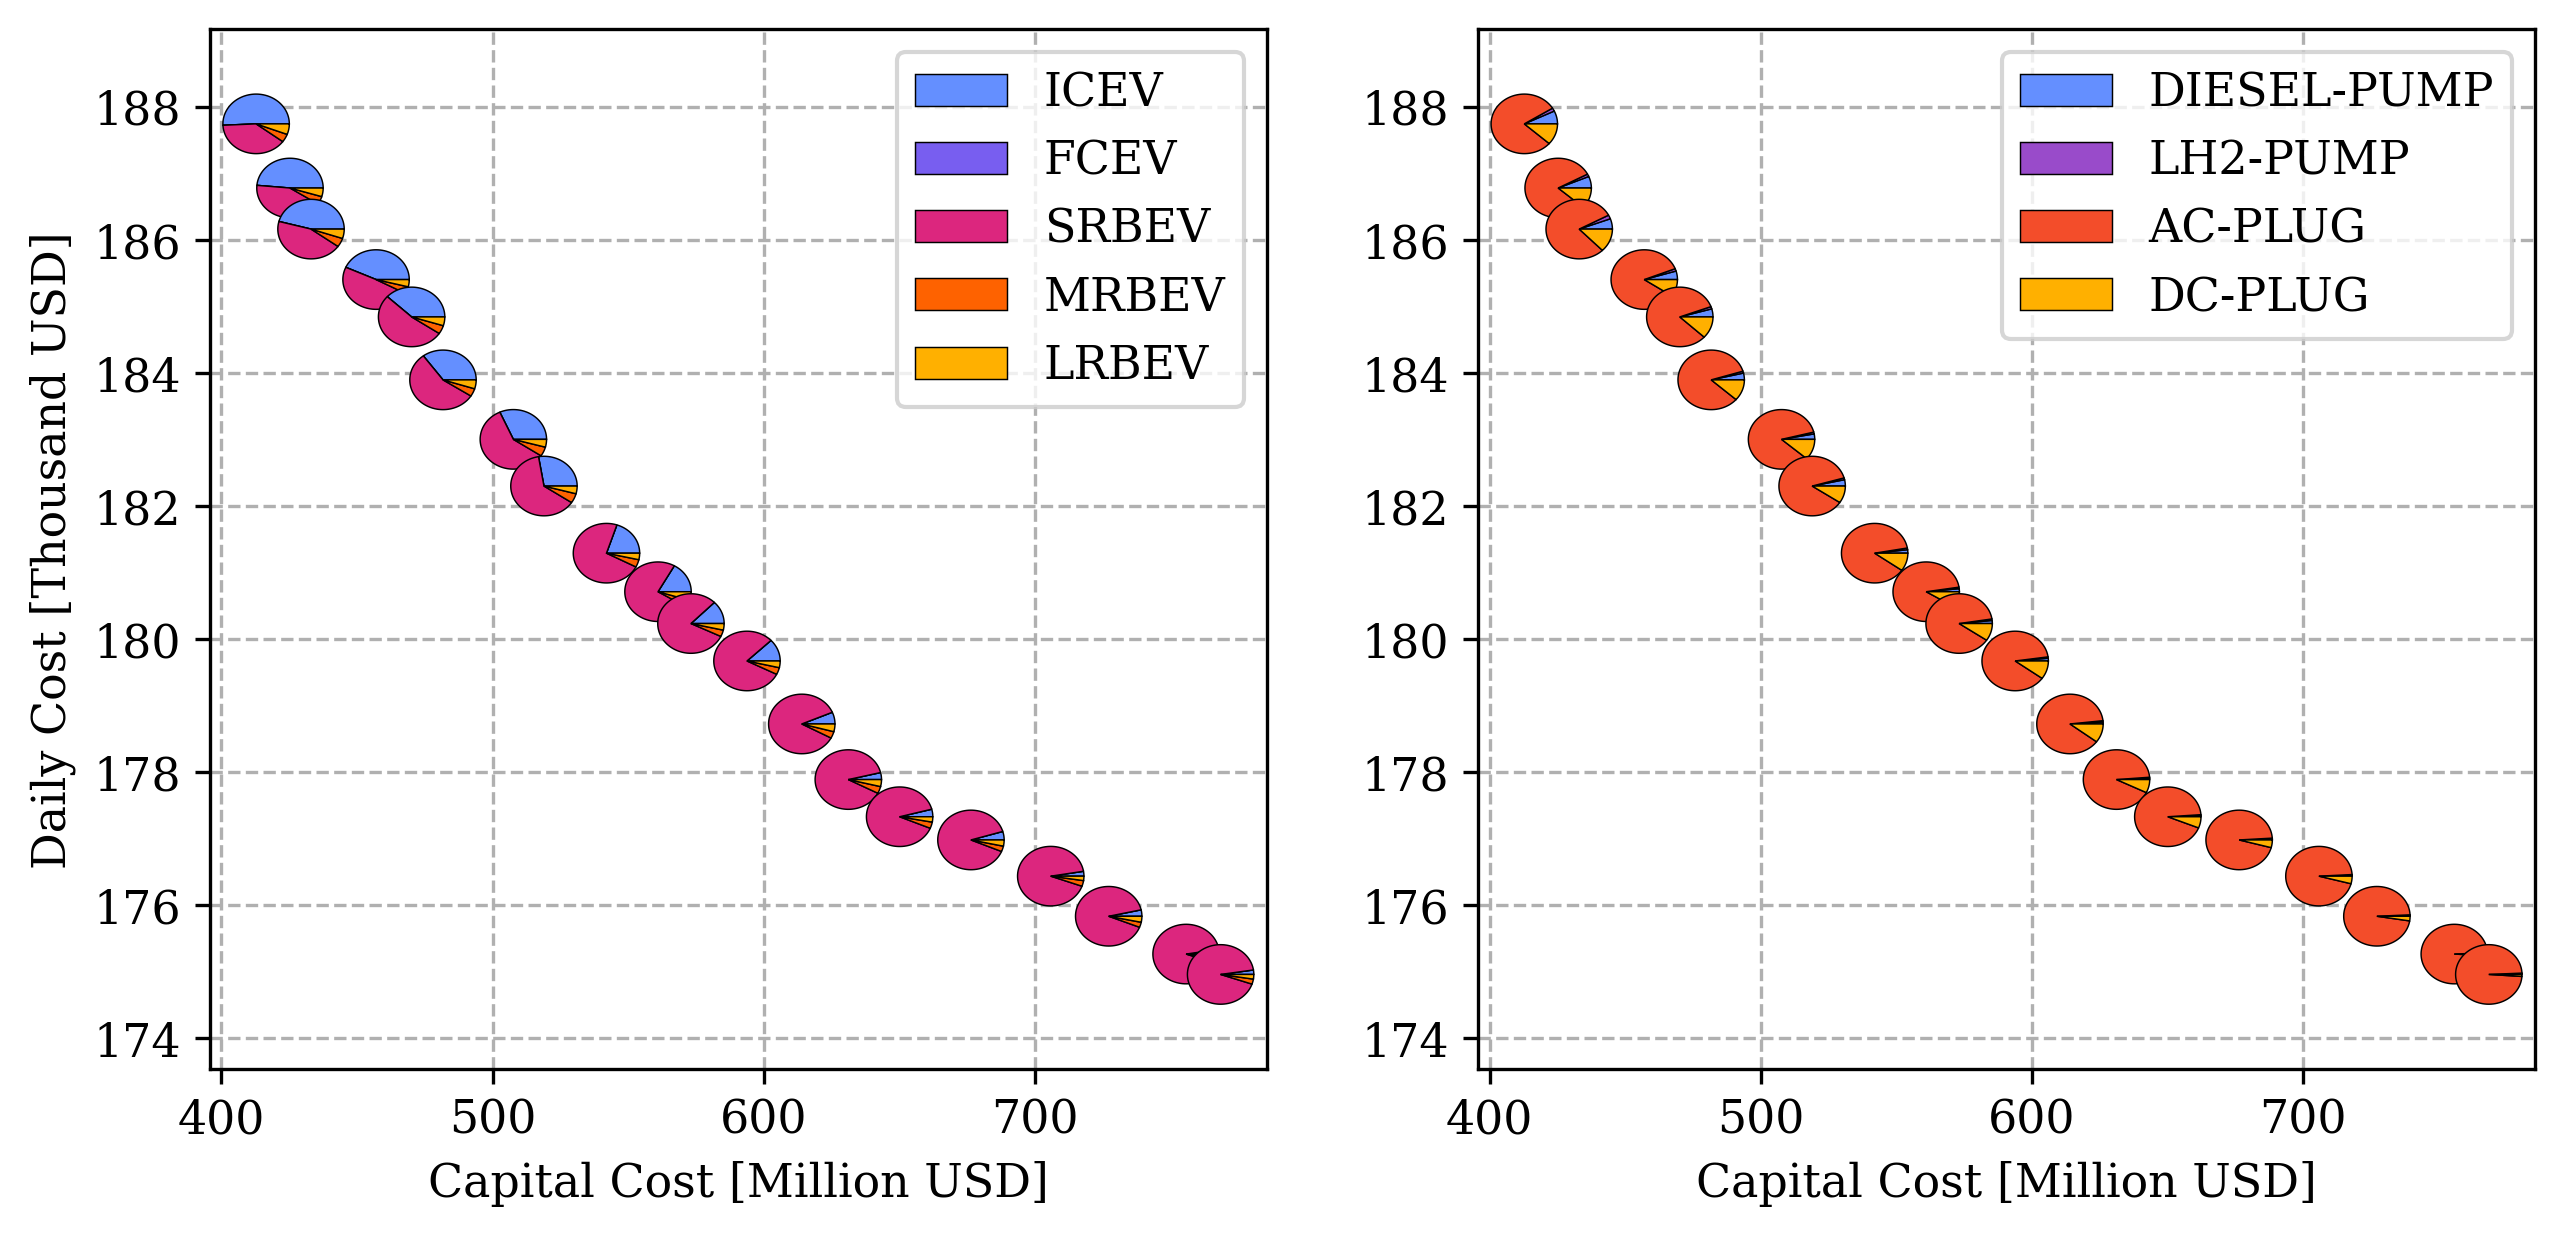
\includegraphics[width = \linewidth]{figs/sfmta_baseline_scatter_pie.png}
	\caption{}
	\label{fig:scatter_pie_baseline_sfmta}
\end{figure}

\begin{figure}[H]
	\centering
	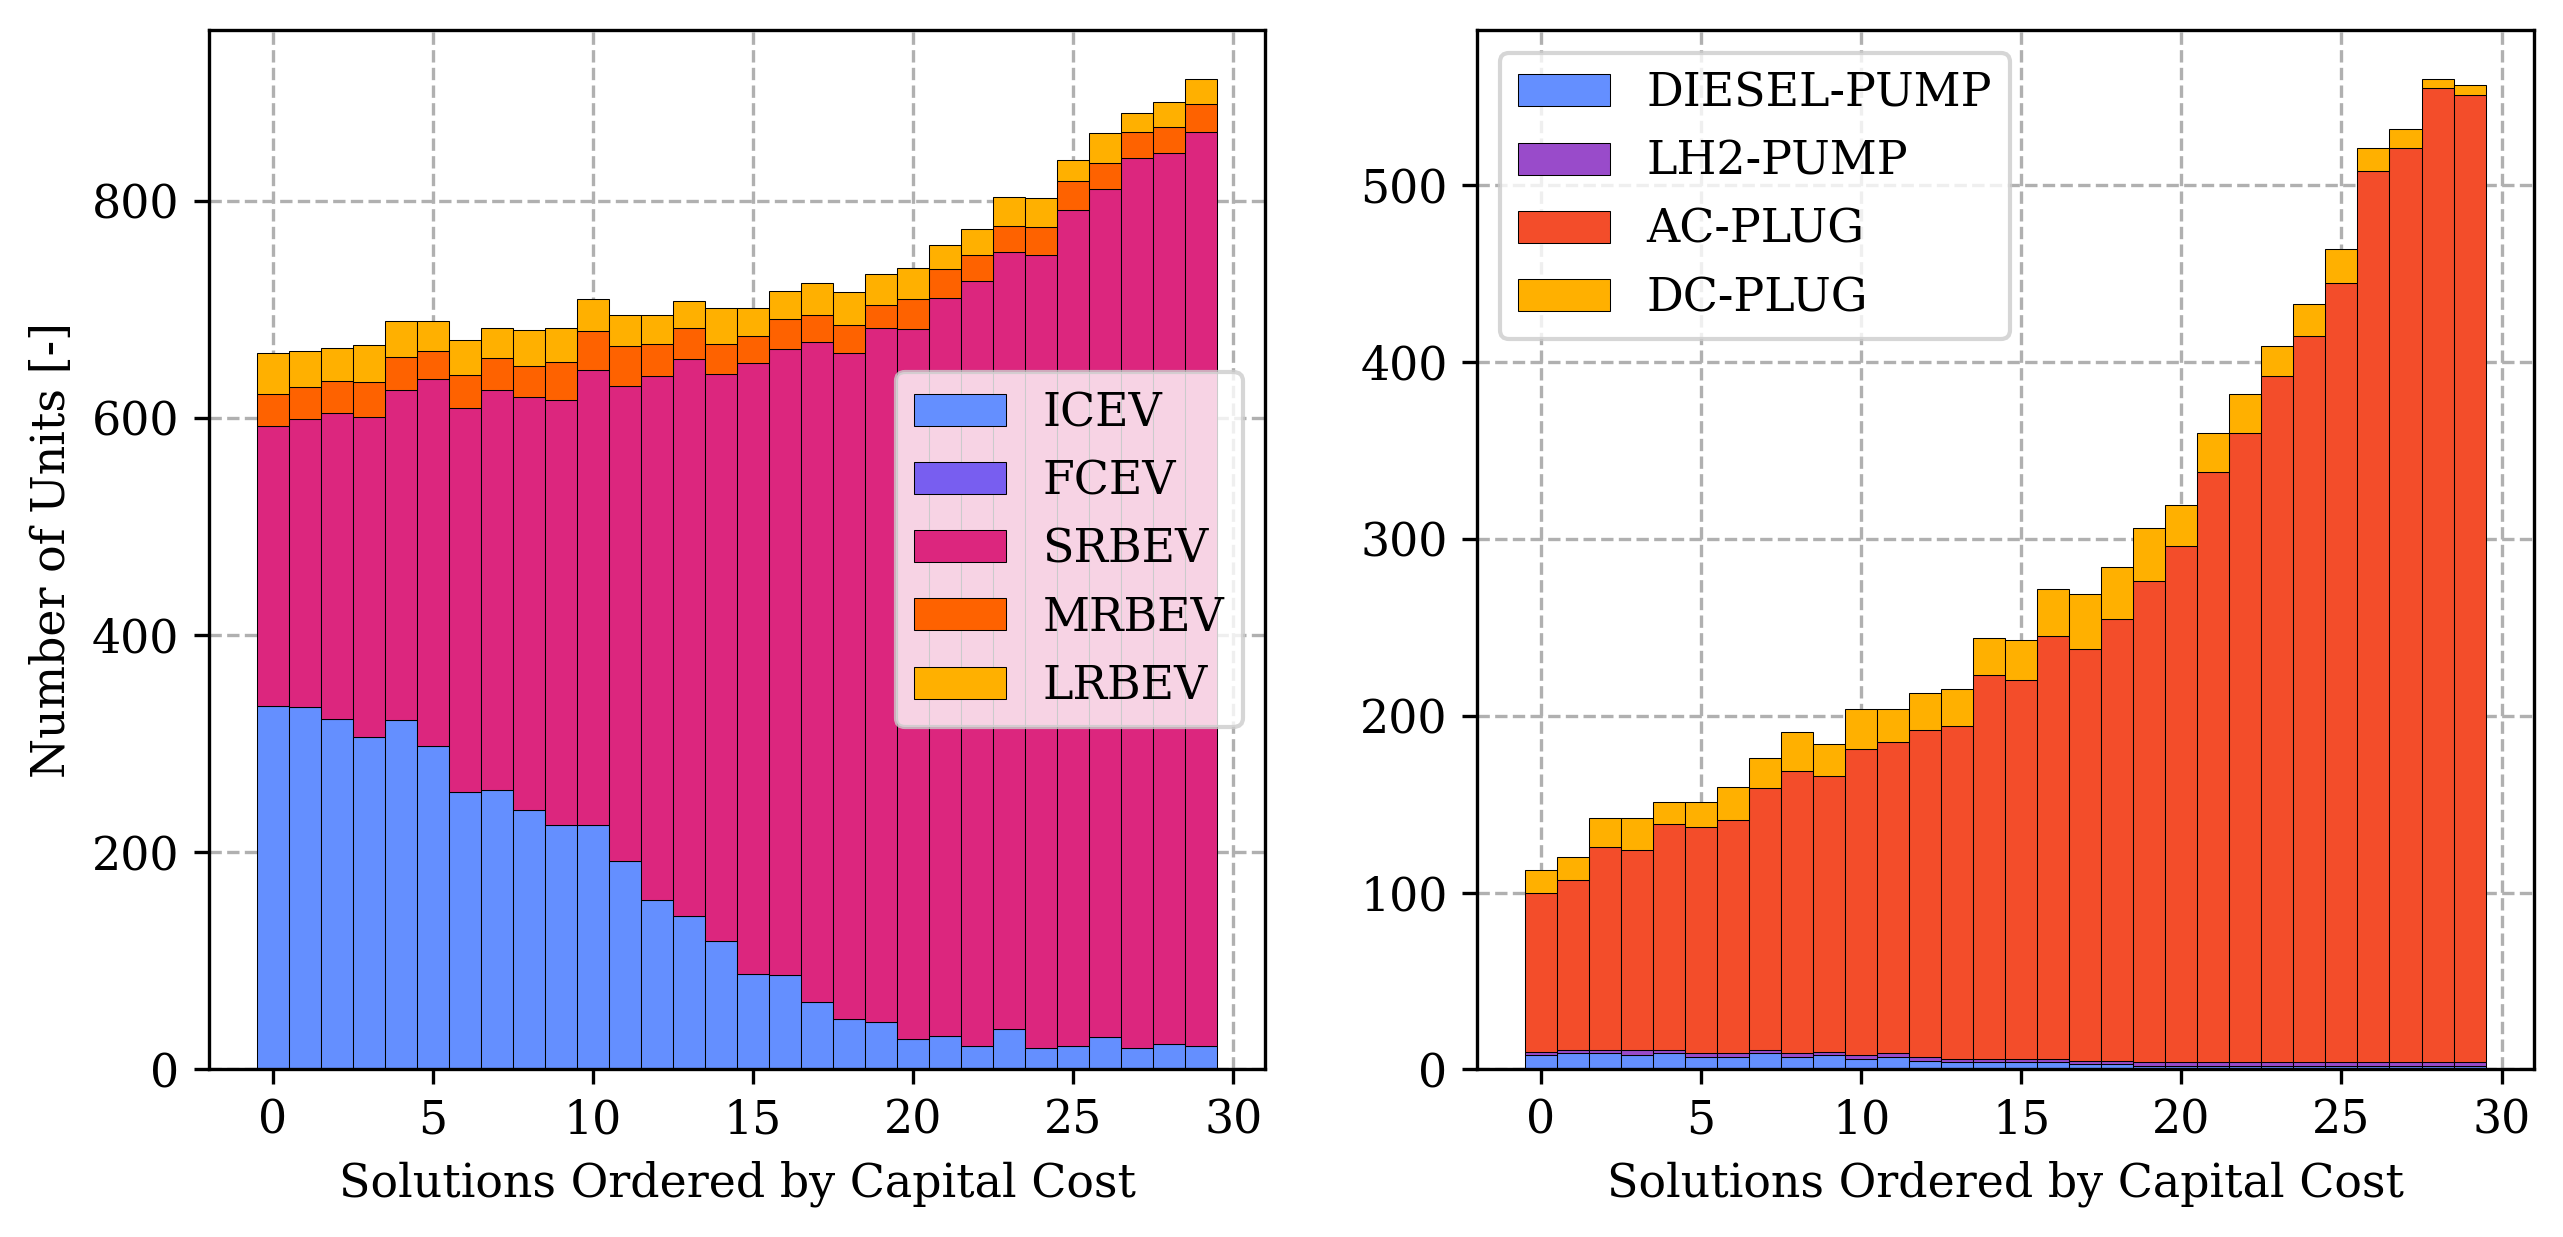
\includegraphics[width = \linewidth]{figs/sfmta_baseline_stacked_bar.png}
	\caption{}
	\label{fig:stacked_bar_baseline_sfmta}
\end{figure}

The actual size of the SFMTA bus fleet is around 850 buses. The solutions produced are in line with this number allowing for the lack of maintenance schedules in the model. The case studies shown here serve to show that the method produces a realistic Pareto front for realistically-scaled networks. The examples used are simplistic in representation of the network (for example neither elevation nor catenary charging were considered), representation of costs, and representation of constraints. All data used in case-study construction is public domain data. The results presented should not be treated as exemplary rather than accurate. Stakeholders applying the method will have much more detailed inputs and, as a result, can obtain accurate solutions. With this information, decision makers can determine what type of fleet to acquire depending on their relative sensitivity to various cost categories. Neither equipment models nor cost functions are integral to the method. More sophisticated and altogether different cost functions and models can be used without changing the core of the method and without changing computational complexity.
	\section{Run-Time Analysis}\label{sec:run_time}

Both the Python and Rust versions of the algorithm were tested comparatively through a structured benchmarking experiment, with the goal of analyzing the similarity in empirical time complexity and solution quality between both implementations across different seeds and input networks. For both code versions, wall-clock timing was recorded for algorithm initialization times (the process of randomly generating an initial solution) and for a 50-generation run, including initialization times. These timings were repeated 15 times per seed, including one discarded ‘warmup round’ to ensure measurements reflect steady-state performance rather than initial overheads. 6 seeds were tested on both implementations, allowing for matched observations and paired analysis between versions with sufficient statistical power. For each seed-version pair, the mean completion time, time per generation, and mean speedup was derived through individual trial data. Time per generation was calculated by subtracting a seed’s mean initialization time from the recorded full time and dividing by 50. The outlined timing experiment was conducted on the Unitrans and SFMTA networks. 

It should be noted that the Rust implementation utilizes multi-threaded parallelism via Rayon for the solution solving task, as opposed to Python’s single-threaded execution. Though theoretically feasible, parallel execution was not considered for the Python implementation due to non-negligible overhead from object serialization across process boundaries. Rayon uses all available logical cores by default, with hardware specifications reported in Table \ref{tab:computer_specs}. The core NSGA-II algorithm is otherwise identical across both implementations and takes the same network input and other hyperparameters as the Python version, relying on PyO3 to provide the Rust bindings for the Python interpreter and Maturin to compile the Rust code and build a standard Python wheel for distribution. This implementation allows for the Rust backend to be utilized directly from a Python environment as a standard importable module, requiring no changes to the existing user-facing interface or practical workflow.

\begin{table}[H]
	\caption{Specifications of computer used for run-time experiment}
	\label{tab:computer_specs}
	\begin{tabular}{|C{.5\linewidth}|C{.5\linewidth}|}
		\hline Component & Specification \\
		\hline CPU & Apple M2 \\
		\hline Core configuration & 8 cores (4 performance + 4 efficiency) \\
		\hline Memory & 16 GB unified memory \\
		\hline L1 cache (I/D) & 128 KB/64 KB \\
		\hline L2 cache & 4 MB \\
		\hline L3 cache & Not present (Apple Silicon uses unified L2) \\
		\hline Clock speed & 3.49 GHz \\
		\hline              
	\end{tabular}
\end{table}

Rust compilation flags include opt-level=3, lto=true, and codegen-units=1. No CPU affinity pinning or process isolation was applied. The OS scheduler was free to migrate threads across all 8 cores. In addition to hardware and software specifications, both the Python and Rust versions of the algorithm were evaluated with the hyperparameters described in Table \ref{tab:hyperparameters}. For timing analysis, Unitrans and SFMTA utilized the same hyperparameters, whereas network-specific hyperparameters were utilized for convergence comparison.

\begin{table}[H]
	\caption{Hyperparameters used for run-time experiment}
	\label{tab:hyperparameters}
	\begin{tabular}{|C{.25\linewidth}|C{.25\linewidth}|C{.25\linewidth}|C{.25\linewidth}|}
		\hline Hyperparameter & \multicolumn{1}{c|}{Timing comparison} & \multicolumn{2}{c|}{Convergence comparison} \\
		\hline &  & Unitrans & SFMTA \\
		\hline Maximum iterations & 50 & 600 & 1000 \\
		\hline Initialization population size & 100 & 500 & 1500 \\
		\hline Core population size & 100 & 150 & 200 \\
		\hline Mutation probability & 0.15 & 0.15 & 0.15 \\
		\hline Crossover probability & 0.5 & 0.5 & 0.75 \\
		\hline Survival threshold & 0 & 0 & 0 \\
		\hline Retries & 50 & 3 & 3 \\
		\hline
	\end{tabular}
\end{table}

\subsection{Timing Results}

The per-network results are given for each seed implementation pair in Tables \ref{tab:timing_unitrans} and \ref{tab:timing_sfmta}. The Shapiro-Wilk test was conducted on each sample to assess the normality of timing distributions, resulting in several statistically significant p-values. This indicates that timing distributions were not consistently normally distributed across trials, which is expected, as timing distributions for iterative algorithms are often right-skewed \cite{Gomes_2000_JAR}. Because of this, non-parametric techniques such as Bootstrapped \glspl{ci} and the Wilcoxon signed-rank test were used for subsequent statistical analysis, as they do not make assumptions about the underlying data distribution. The Wilcoxon signed-rank test was chosen to analyze paired Python-Rust timings for statistically significant differences. A 95\% \gls{ci} with 9,999 resamples was utilized for all intervals constructed, and all bootstrap resampling was completed with the same random state. A statistically significant time performance difference was found between the Python and Rust implementations for the initialization and full runs of the Unitrans and SFMTA networks

\begin{table}[H]
	\caption{Run-time results for Unitrans example network}
	\label{tab:timing_unitrans}
	\begin{tabular}{|C{.1428\linewidth}|C{.1428\linewidth}|C{.1428\linewidth}|C{.1428\linewidth}|C{.1428\linewidth}|C{.1428\linewidth}|C{.1428\linewidth}|}
		\hline \multicolumn{1}{|c|}{Seed} & \multicolumn{2}{c|}{Initialization (s)} & \multicolumn{2}{c|}{Full Run (s)} & \multicolumn{2}{c|}{Time/Generation (s)} \\
		\hline Language & Python & Rust & Python & Rust & Python & Rust \\
		\hline 0 & 3.332 (0.035) & 0.183 (0.0007) & 94.39 (0.138) & 4.203 (0.019) & 1.821 & 0.080 \\
		\hline 1 & 3.316 (0.051) & 0.185 (0.004) & 93.05 (0.084) & 4.216 (0.017) & 1.795 & 0.081 \\
		\hline 2 & 3.313 (0.033) & 0.185 (0.001) & 91.83 (0.410) & 4.216 (0.051) & 1.770 & 0.082 \\
		\hline 3 & 3.445 (0251) & 0.185 (0.008) & 94.45 (0.215) & 4.201 (0.027) & 1.820 & 0.080 \\
		\hline 4 & 3.337 (0.032) & 0.184 (0.001) & 93.75 (0.141) & 4.287 (0.027) & 1.808 & 0.082 \\
		\hline 5 & 3.317 (0.064) & 0.183 (0.002) & 93.66 (0.130) & 4.260 (0.042) & 1.807 & 0.082 \\
		\hline
	\end{tabular}
\end{table}

\begin{table}[H]
	\caption{Run-time results for SFMTA example network}
	\label{tab:timing_sfmta}
	\begin{tabular}{|C{.1428\linewidth}|C{.1428\linewidth}|C{.1428\linewidth}|C{.1428\linewidth}|C{.1428\linewidth}|C{.1428\linewidth}|C{.1428\linewidth}|}
		\hline \multicolumn{1}{|c|}{Seed} & \multicolumn{2}{c|}{Initialization (s)} & \multicolumn{2}{c|}{Full Run (s)} & \multicolumn{2}{c|}{Time/Generation (s)} \\
		\hline Language & Python & Rust & Python & Rust & Python & Rust \\
		\hline 0 & 14.49 (0.083) & 0.628 (0.008) & 483.2 (0.462) & 24.59 (0.088) & 9.374 & 0.479 \\
		\hline 1 & 14.52 (0.101) & 0.632 (0.008) & 486.3 (0.497) & 24.83 (0.073) & 9.435 & 0.484 \\
		\hline 2 & 14.55 (0.052) & 0.622 (0.006) & 489.2 (0.537) & 25.14 (0.103) & 9.494 & 0.490 \\
		\hline 3 & 14.55 (0.161) & 0.620 (0.011) & 486.9 (2.844) & 25.25 (0.095) & 9.447 & 0.493 \\
		\hline 4 & 14.50 (0.062) & 0.626 (0.006) & 486.2 (0.450) & 25.14 (0.110) & 9.434 & 0.490 \\
		\hline 5 & 14.51 (0.051) & 0.630 (0.005) & 488.9 (1.766) & 25.03 (0.323) & 9.488 & 0.488 \\
		\hline
	\end{tabular}
\end{table}

\subsection{Convergence Comparison}

Convergence quality was assessed using the hypervolume indicator, which is defined as the volume of objective space dominated by the Pareto front and bounded by a reference point set to 110\% of the worst observed objective values across all runs. A higher hypervolume indicates a larger, better-spread front. Paired hypervolumes across seeds was evaluated for both the Unitrans and SFMTA networks to compare the rate, quality, and similarity of convergence across implementations. For convergence testing, the max_iter hyperparameter was set to 600 for Unitrans, and 1,000 for SFMTA. Convergence was determined via the retries parameter, which was set to 3. The retries parameter terminates the evolution process early if no updates to the chosen population are made within a certain number of attempts. Figure \ref{fig:hypervolume_convergence} highlights the convergence via hypervolume for Python and Rust implementations across all seeds, showing mean hypervolume per generation $\pm 1$ standard deviation. Average hypervolume remains similar over generations, indicating consistency across algorithms. All solutions ran to convergence.

\begin{figure}[H]
	\centering
	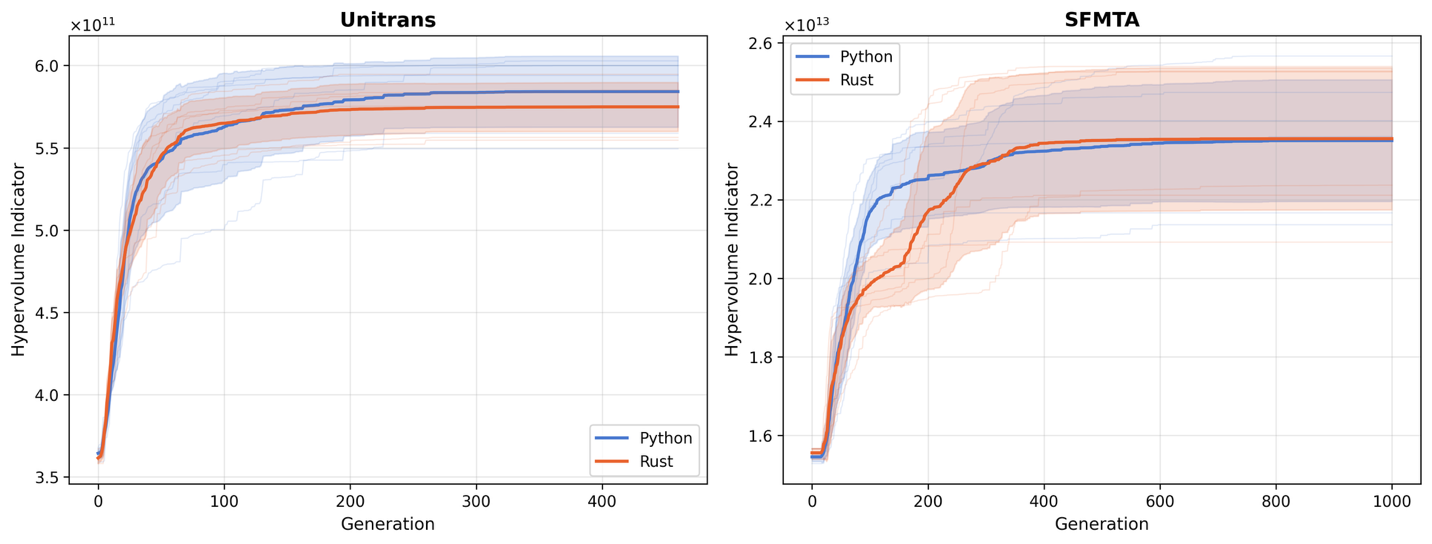
\includegraphics[width = \linewidth]{./figs/hypervolume_convergence.png}
	\caption{Evolution of hypervolume by generation for Python and Rust implementations for Unitrans and SFMTA networks.}
	\label{fig:hypervolume_convergence}
\end{figure}

Two Wilcoxon signed-rank tests were conducted on the paired Python-Rust hypervolumes for Unitrans and SFMTA, with p-values of 0.5625 and 1.0000, respectively. These results are displayed in Figure \ref{fig:hypervolume_boxplots}. This indicates that there is no statistically significant difference between the hypervolumes produced across seeds in either implementation.


\begin{figure}[H]
	\centering
	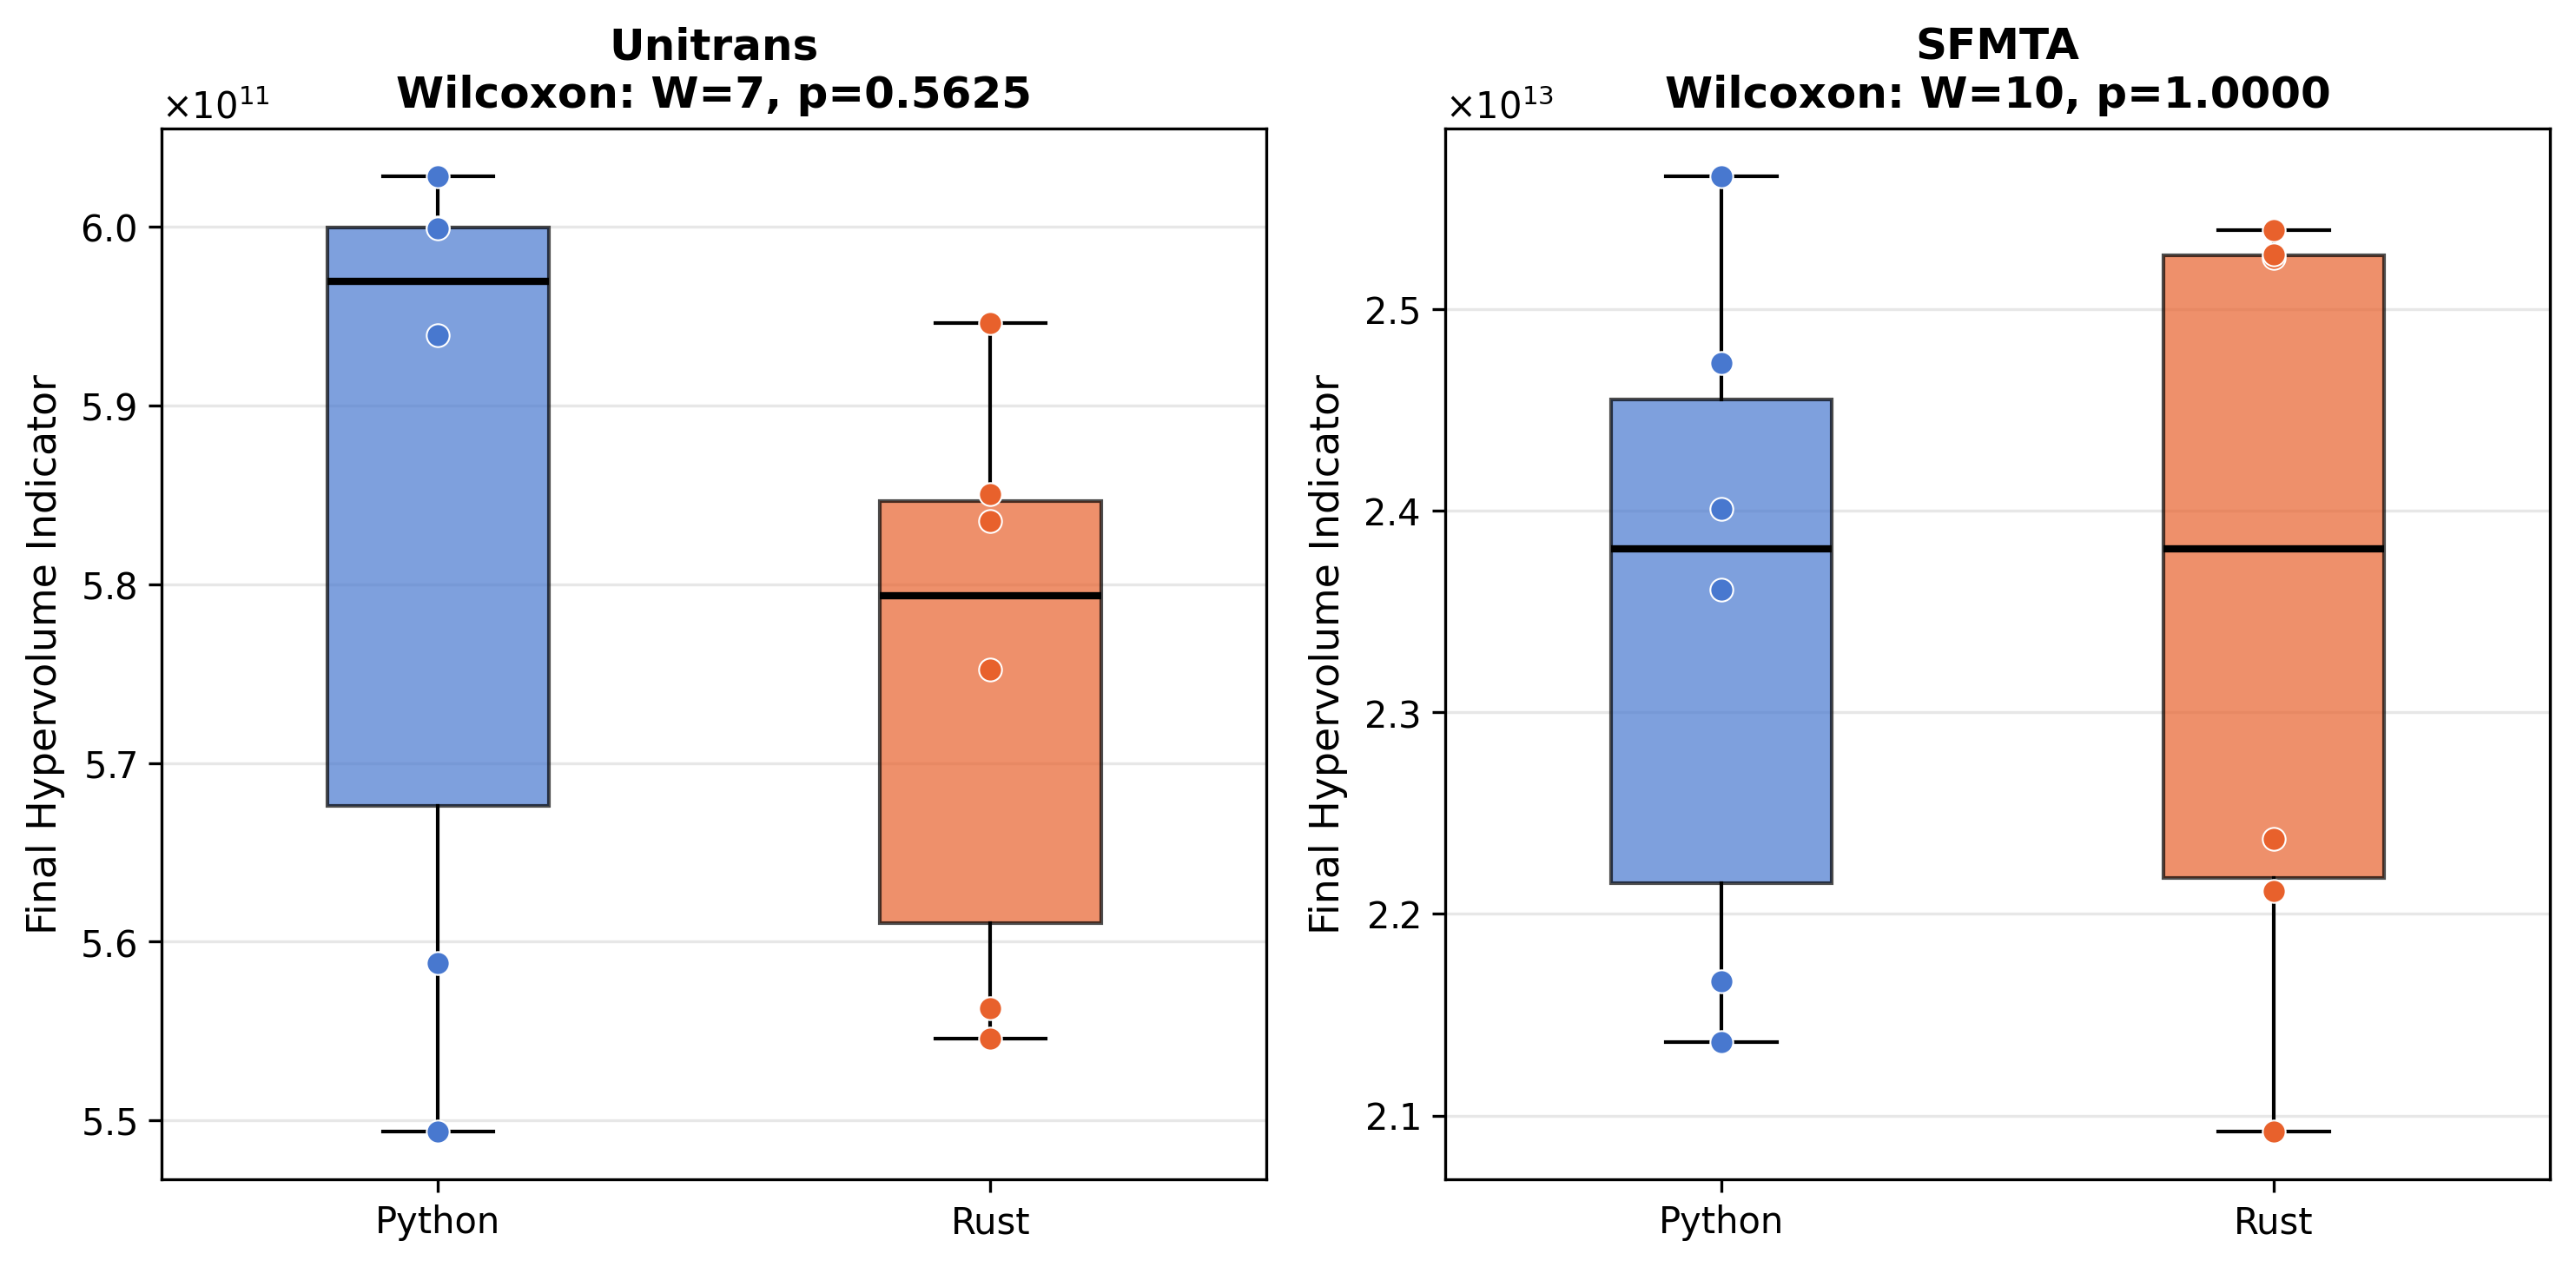
\includegraphics[width = \linewidth]{./figs/hypervolume_boxplots.png}
	\caption{Boxplots of final hypervolume for Python and Rust implementations for Unitrans and SFMTA networks.}
	\label{fig:hypervolume_boxplots}
\end{figure}
	\section{Conclusions}

As transit bus operators face difficult decisions on designing their future fleets, decision support tools are of tremendous value. Designing a future fleet requires solving the \gls{vsfmp} which is known to be a NP-hard \gls{cop}. Solving the \gls{vsfmp} using an optimal solver requires evaluation of a set of integer trip-to-trip adjacency matrices (one for each bus type) and a set of supply-event=to-supply-event adjacency matrices (one for each supply port type). This complexity renders the problem effectively unsolvable for networks of realistic scale. Solving returns a single optimum which is useful for operational purposes but less so for strategic decision making. Strategic decision makers are better informed when they are able to see the trade-offs between objectives and how these manifest in fleet design.

This study alleviates this issue by presenting a flexible, efficient Pareto optimization algorithm for the \gls{vsfmp}. The \gls{nsga} framework utilized allows for a Pareto front to be revealed in N dimensions. The computational efficiency of the algorithm allows for reasonably quick iteration even using ordinary desktop or laptop computers which will be readily available to technical employees. The utility of the algorithm is demonstrated for medium and large bus networks in Section \ref{sec:case_study} efficiency and repeatability of the algorithm is demonstrated in Section \ref{sec:run_time}. Overall, the methodology presented in this paper, and implemented in the associated repository, provides transit agencies with a novel and usable tool to help them make their toughest decisions.

\subsection{Limitations and Future Work}

The methodology presented shares limitations with other metaheuristic methods and especially other \gls{nsga} based methods. Namely, it is not possible to know if a true optimum has been reached or if the solution arrived at is dictated by hyperparameters or even random seeding. Any \gls{nsga} method bears the specific issue that maintenance of field spread can only be guaranteed with impractically large population sizes. The method presented here mitigates this issue by allowing for a larger initial population and, thus, initial variety in solutions. Analysis of convergence across seeds shows that consistency is possible but hyperparameters may need to be tuned by network. Future work will include the development of objectives and constraints that match the real-life considerations of transit operators, more realistic models of both networks and equipment, and further work towards solution consistency including hyperparameter studies and alternate strategies such as population-migration.

\section{CRediT Statement}

\noindent\textbf{Aaron Rabinowitz:} Conceptualization, Methodology, Writing - Original Draft, Visualization, Software. \textbf{Jeremy Elvander:} Data Curation, Software, Writing - Original Draft. \textbf{Vaishnavi Karanam:} Conceptualization, Writing - Review \& Editing, Funding Acquisition, Project Administration. \textbf{Gil Tal:} Supervision, Funding Acquisition, Writing - Review and Editing.
	
	\bibliographystyle{elsarticle-harv}
	\bibliography{./sources/combined.bib}
		
\end{document}